\section{Genetic Algorithms}
\label{sec:eval:GAs}

The core of my approach to solving the problems outlined in Chapter~\ref{chap:Intro} was creating a Genetic algorithm to evolve populations of candidate routes, returning the fittest once the termination criteria are met.

GAs are transparent but stochastic approaches to optimisation problems. As such, it is much easier to examine the operations and decisions they make compared with \textit{black box} approaches such as neural networks, however due to their random nature, it can be difficult to predict their exact behaviour and results can differ greatly from run to run if the number of generations or population size is too low.

Whilst a poor choice of training data can lead to unintended/ unpredictable behaviour from approaches like neural networks, they have the advantage that most of their compute time is used when constructing the initial model, subsequent usage of these models requires little compute time. Whereas, GAs must run the entirety of the \textit{learning} process from scratch whenever a new route or set of routes is required. In an application where the system sees a high number of unique requests, this compute time can quickly amount to much longer than the training time for a neural network.

\subsection{Genetic Operator Performance}

During development I implemented two different operators in each category, but there are many other approaches proposed in academic literature. Given more time, I would have liked to implement more and present a more empirical evaluation of each.

\subsubsection{Selection}

In a single generation, over three populations of 15 individuals, my ranked selection operator ran 3 times totalling $75.1\mu s$ or an average of $25 \mu s$ per run, a negligible amount of time relative to the overall runtime.

As you can see in Figure~\ref{fig:selection_eg}, my ranked selection operator performs its task well, removing the obviously less fit individuals in favour of more copies of  fitter ones. This can be seen by the removal of the line that dips below the $x$ axis (in this example the bottom road boundary was defined as $b_{1}(x) = 0 $) and the fact that duplicate routes are found as indicated by the 3rd graph of unique routes showing fewer individuals than the second.

Ranked selection compared with fitness proportional (roulette wheel selection) is much more predictable, it may not explore as much of the search space but it is more likely to thoroughly explore a single area. Most other selection operators seem to focus on maintaining a diverse population so as to not get stuck in local minima.

\subsubsection{Mutation}

The mutation operators I implemented were Uniform and Gaussian.

I found Gaussian to perform better in cases where a route may be close to optimal in the phenotypic space, i.e. with minimal changes to trajectory, it would be optimal. In such cases the genotypic fitness may not accurately represent this, a route that collides with another or passes through infeasible space will suffer from a large genotypic fitness penalty possibly encouraging it to be removed from the \textit{gene pool}. Gaussian mutation, preferring mutated points closer to their initial position can be effective as moving such routes closer to the optima.

However, in cases where the initial population generation has created all routes far from the optimal, Gaussian mutation can struggle to generate mutated points extreme enough to direct the GA towards the minima.

Part of the problem with Gaussian mutation, and mutation in general on $n$-degree Bezier curves, is that even a relatively major control point movement may cause only minor changes to the overall trajectory of the curve in cases where $n$ is high.

An example of a relatively large control point mutation leading to a minor direction change can be seen in Figure~\ref{fig:gauss_mutation_eg}.

It is possible that an approach incorporating a form of Simulated Annealing could help to broadly explore the search space in early generations before refining solutions in a found minima in latter generations. This could operate by applying a different mutation operator such as Uniform mutation in the first 60\% of generations before swapping to Gaussian when we would expect our algorithms to have found some local minima.

In a single generation, over the same 3 sets of 15 individuals, my Gaussian mutation operator ran 3 times totalling $1.71 ms$ runtime, an average of $571\mu s$. This is an insignificant amount of time when compared to the overall runtime of this task which stands at $14.4$.

\subsubsection{Crossover}

I implemented both single point and $k$ point crossover. I ran my benchmarks using single point crossover in an attempt to minimise the amount of randomness and differences in convergence speed between samples.

\todo{Implement another crossover operator to talk about ?}

\subsubsection{Fitness}

As previously mentioned the most important operator, and the one I spend the most time working on, is the fitness function.

This acts as the objective function for the algorithm as it seeks to minimise its value across multiple agents over multiple generations.

This operation, especially when modified to detect collisions, was the source of most of the runtime of my project. In the toy example of 3 sets of 15 agents across a single generation, the fitness function accounted for a large proportion of the runtime at $14.4$ across 3 calls, an average of $4.81$ seconds per invocation. This is after all my attempts to speedup the process (See Section~\ref{subsec:approach:bezInt}).

The final incarnation of my fitness function can be thought of as two separate parts:

\begin{enumerate}
  \item The \textit{base fitness} i.e. the fitness when considered in isolation in the road space.

        This calculation again can be thought of as being comprised of 3 parts as outlined in Equation~\ref{eq:basefitness}:

        In total this portion of the function ran 135 times in an average of $55.9ms$ for a total of 52.3\% of the fitness function runtime

        \begin{enumerate}
          \item Route length

                This procedure had an average runtime of around $5.36\mu s$, running 135 times it amounted for $0.01$\% of the fitness function runtime.

          \item Infeasible distance length taking an average of $32.7ms$ to run over its 135 runs, making up $30.6$ of the fitness function runtime.
          \item Close proximity distance length took an average of $23.2ms$ over 135 runs totalling $21.7$\% of the runtime

        \end{enumerate}


  \item The collision penalty

        Collision detection as previously stated was a major source for complexity in my project. However, after a lot of tweaking and time saving measures, in this toy example the runtime for the collision detection stands at an average of $24.8$ms, around the same as the runtime of the high proximity distance calculation.
\end{enumerate}\todo{Is this all too boring?, come back to this }


\section{Bézier Curves}
\label{sec:eval:bezier}

Bézier curves have been utilised in this project to encode and represent the route of a vehicle. As mentioned in Section~\ref{sec:back-bezier-curves}, there are many reasons I originally selected them for this task. However, over the course of implementation and testing, a number of downsides have been presented.

\begin{enumerate}
  \item Objective\todo{correct word?} numerical approaches with Bézier curves are often complicated, expensive and do not generalise well to $n$ control points.

        This leads to many heuristics, and approximations being employed to save computation. Approximations and assumptions in a system as the one proposed in this report, are sub-optimal and could potentially lead of undesired behaviour which could ultimately have dire consequences if such a system were to be deployed.

        Other research such as that by Cai \& Peng\cite{caiCooperativeCoevolutionaryAdaptive2002} takes a different approach, using discrete, grid-based search spaces in which routes are made up of a series of connected straight line segments. This approach removes much of the complexity from my solution but introduces its own concerns.

        The routes generated by Cai \& Peng's approach are intended to be executed by autonomous robots, so no thought has been given to potential passengers. Consequently, these routes would require smoothing as a post-planning process, re-introducing complexity.

        Another possible representation is the approach taken by Cruz-Piris et al.\cite{cruz-pirisAutomatedOptimizationIntersections2019} which involved representing the section of road, in their case an intersection, as a cellular automata in which a single vehicle can occupy a single cell at any given point in time. \end{enumerate}\todo{does this need to be an enumerated list?}


There were however, also some advantages and nice properties of Bézier curves which lent themselves to the task.

Their relatively simple abstract construction as a series of control points proved easy to concretely represent as a genotype. This made the creation of the various genetic operators relatively simple, requiring little pre or post-processing.

They are also capable of representing a high complexity of curve in a relatively simple and concise manner. This makes code much more approachable and algorithms easier to digest.

\section{Single Agent Planning}\todo{go back and talk about solution complexity + planning time in more detail}

The majority of the components of my single agent planning system have been evaluated in Sections~\ref{sec:eval:GAs} and \ref{sec:eval:bezier}. Here I will discuss its overall effectiveness and any possible extensions that could be implemented given more time.


\begin{figure}[ht]
  \centering
  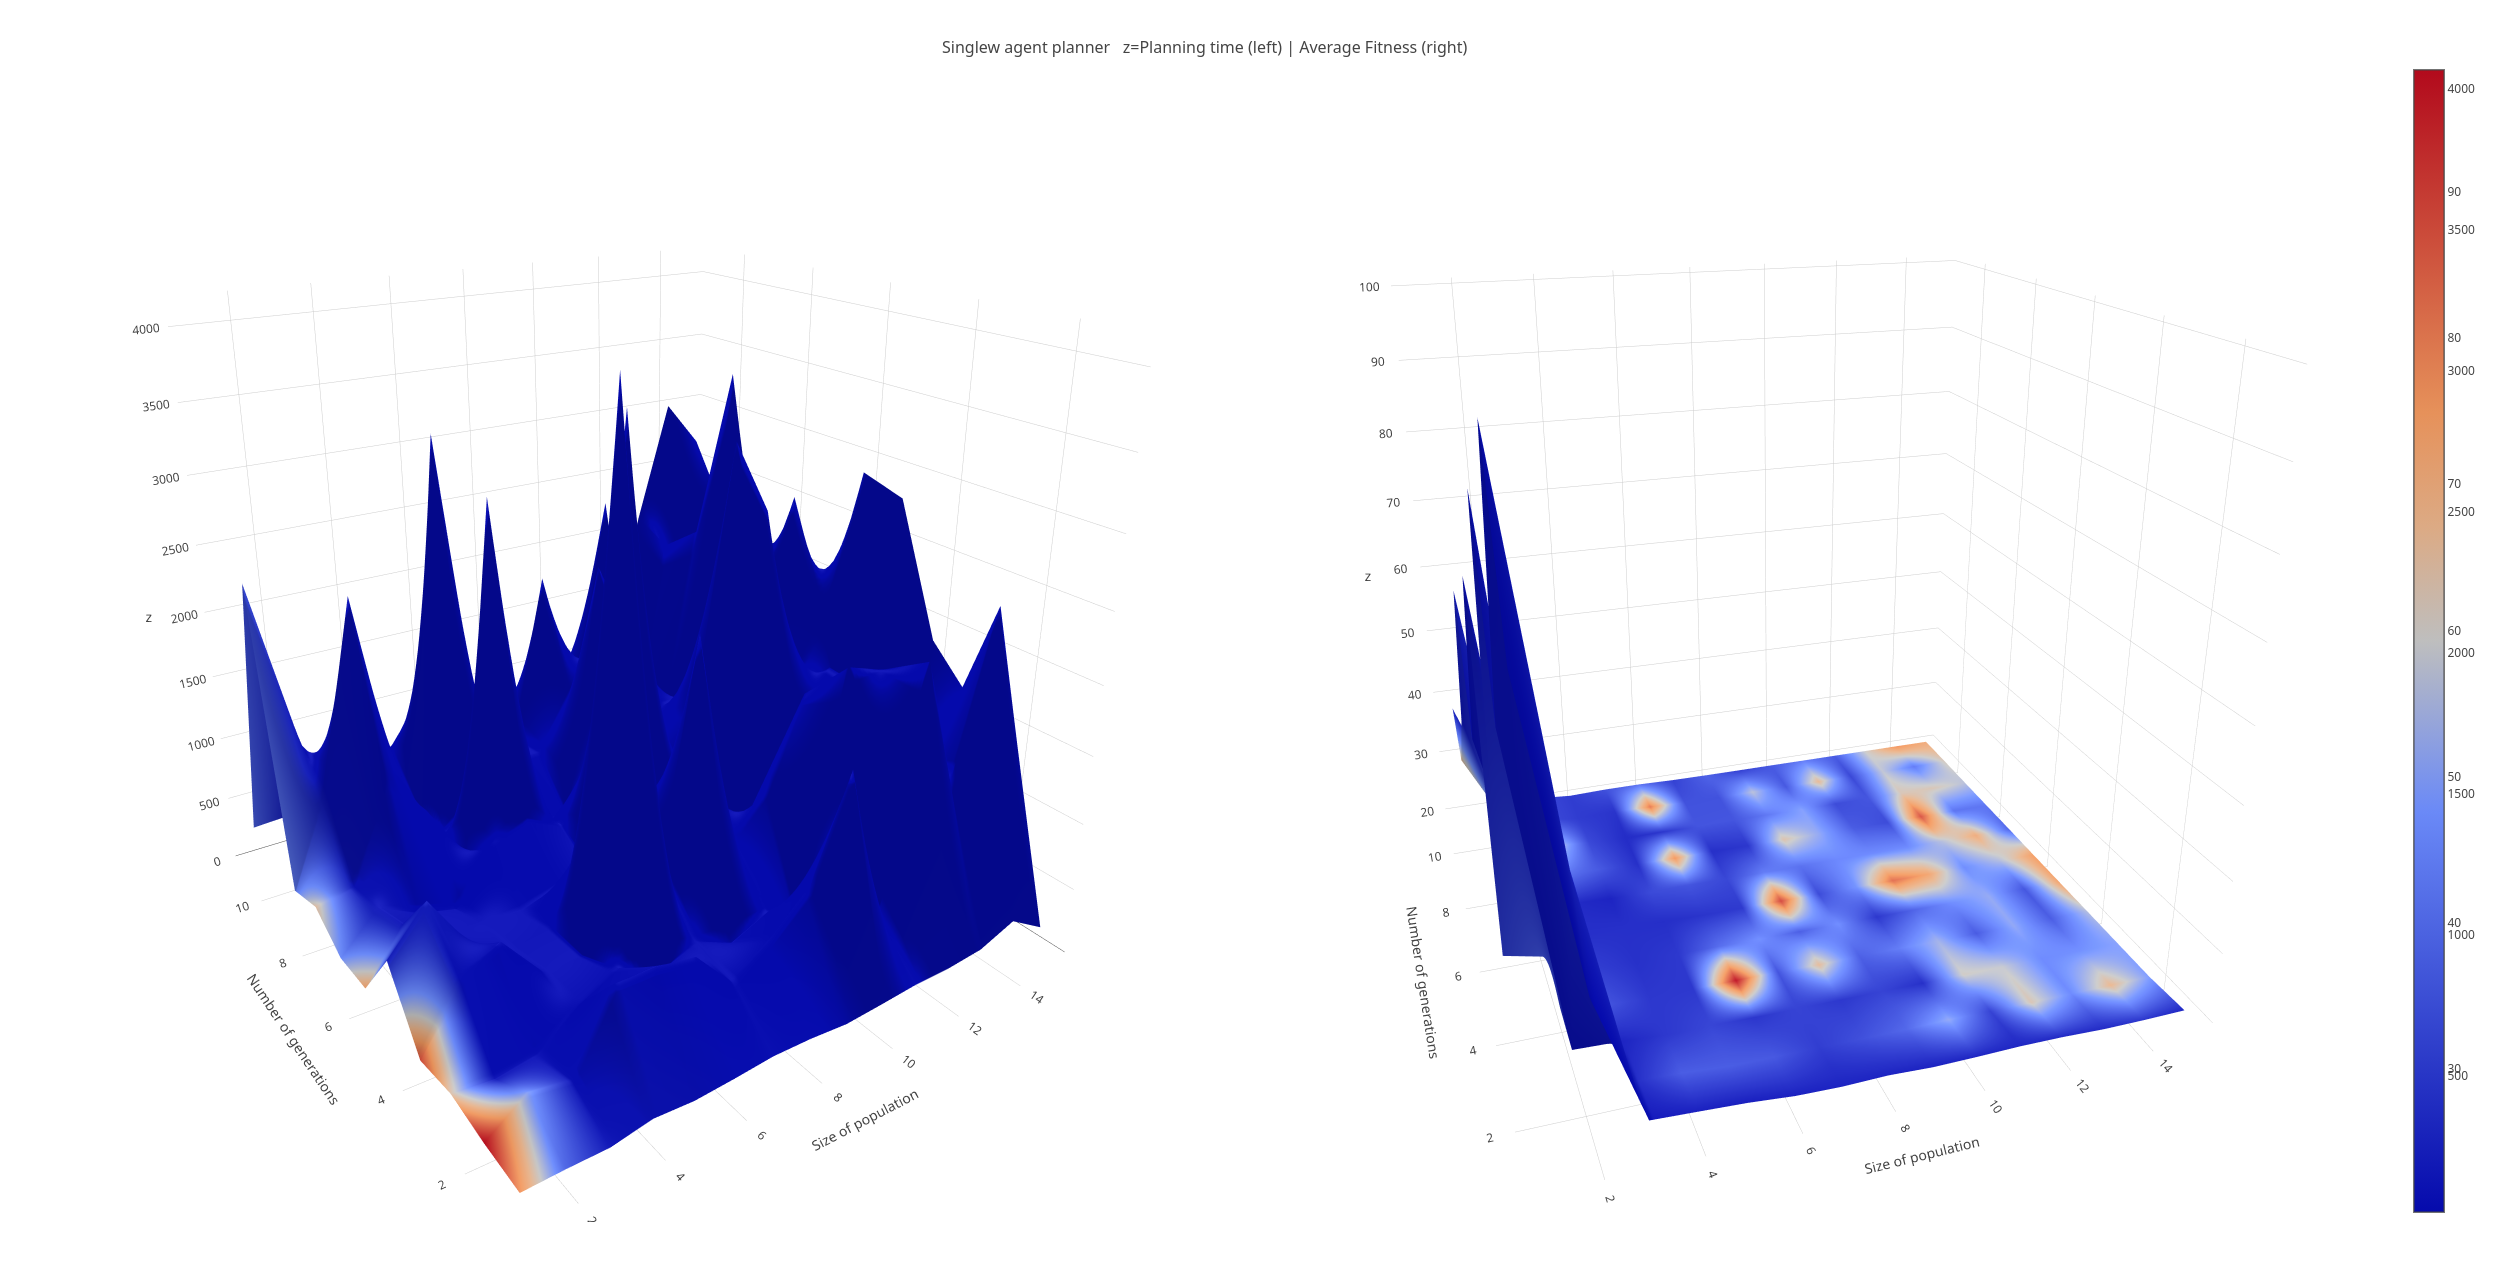
\includegraphics[scale=0.14]{figures/sa-1404-col.png}
  \caption{\label{fig:sa-col} Single agent planning: number of generations against size of population against planning time (left), fitness (right), over \textit{easy} road space (Figure~\ref{subfig:sa-road1})}
\end{figure}\todo{replot with seconds on z axis}

\begin{figure}[ht]
  \centering
  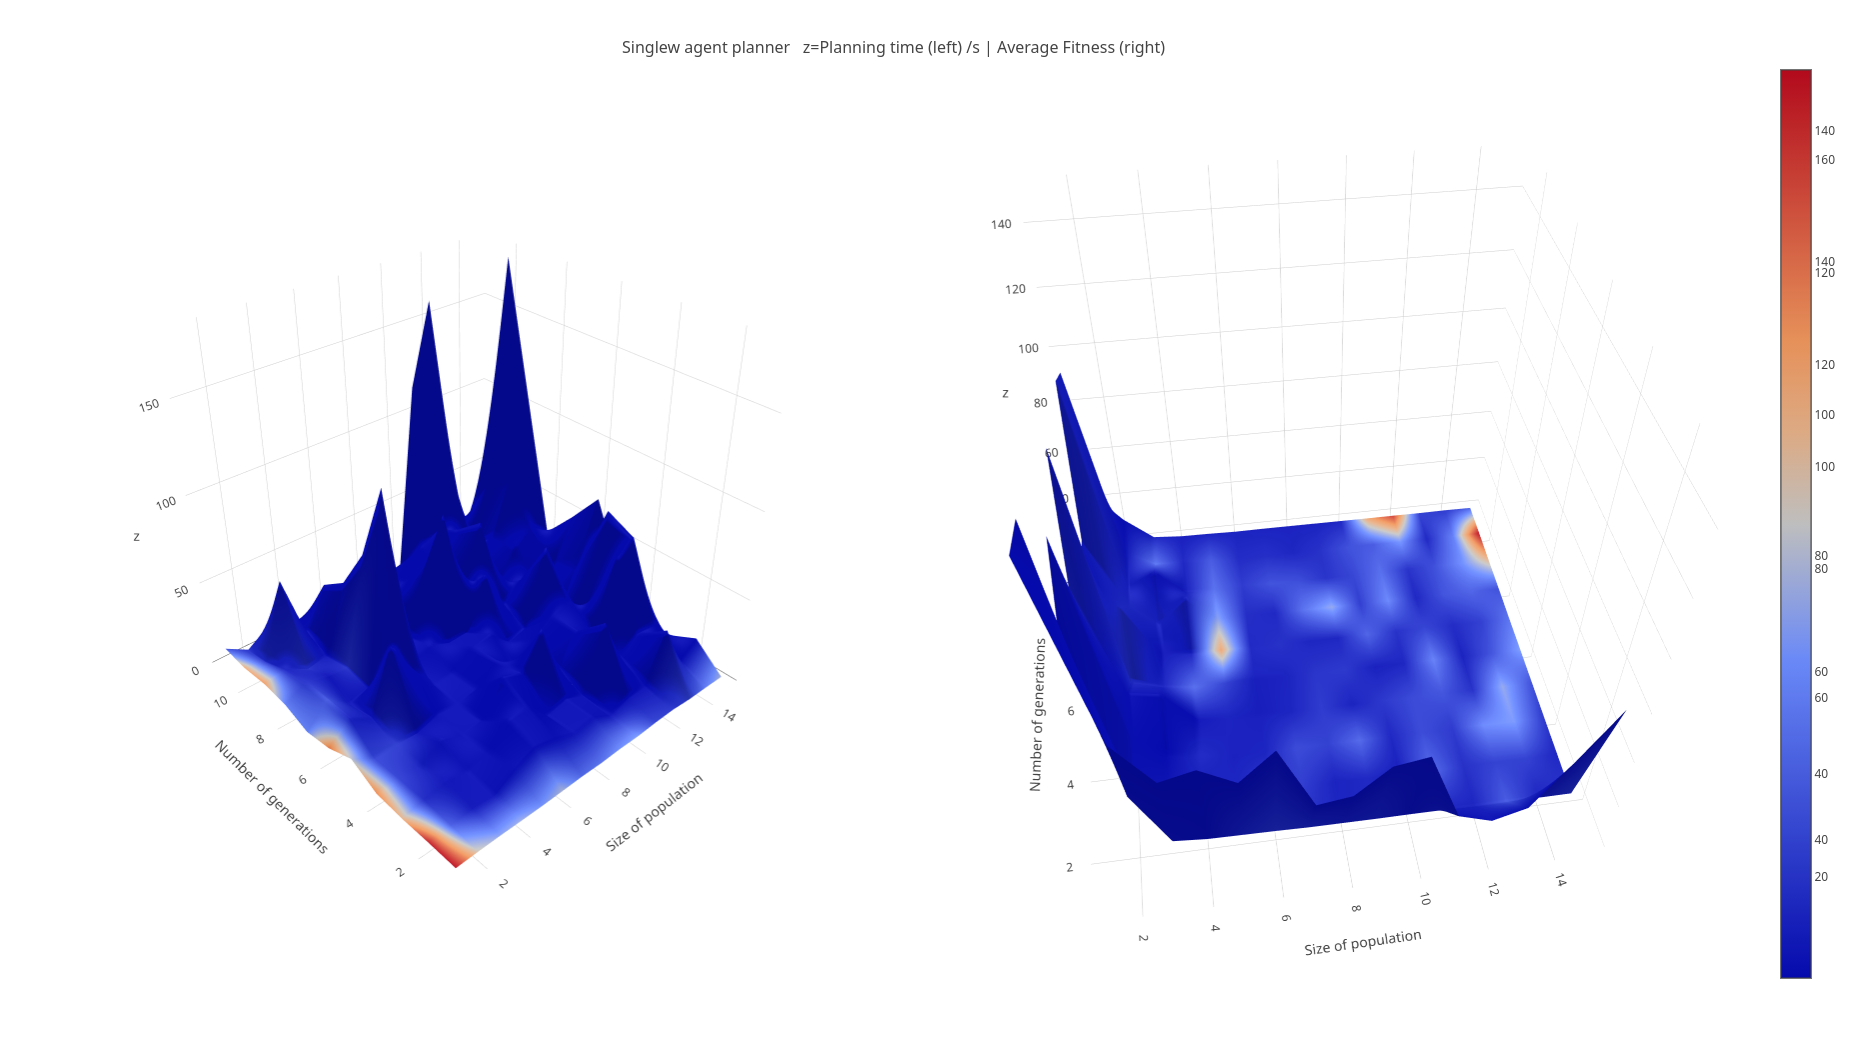
\includegraphics[scale=0.2]{figures/sa-diff2.png}
  \caption{\label{fig:sa-diff2} Single agent planning: number of generations against size of population against planning time (left) /s, fitness (right), over \textit{moderately difficult} road space (Figure~\ref{subfig:sa-road2})}
\end{figure}

\begin{figure}[ht]
  \centering
  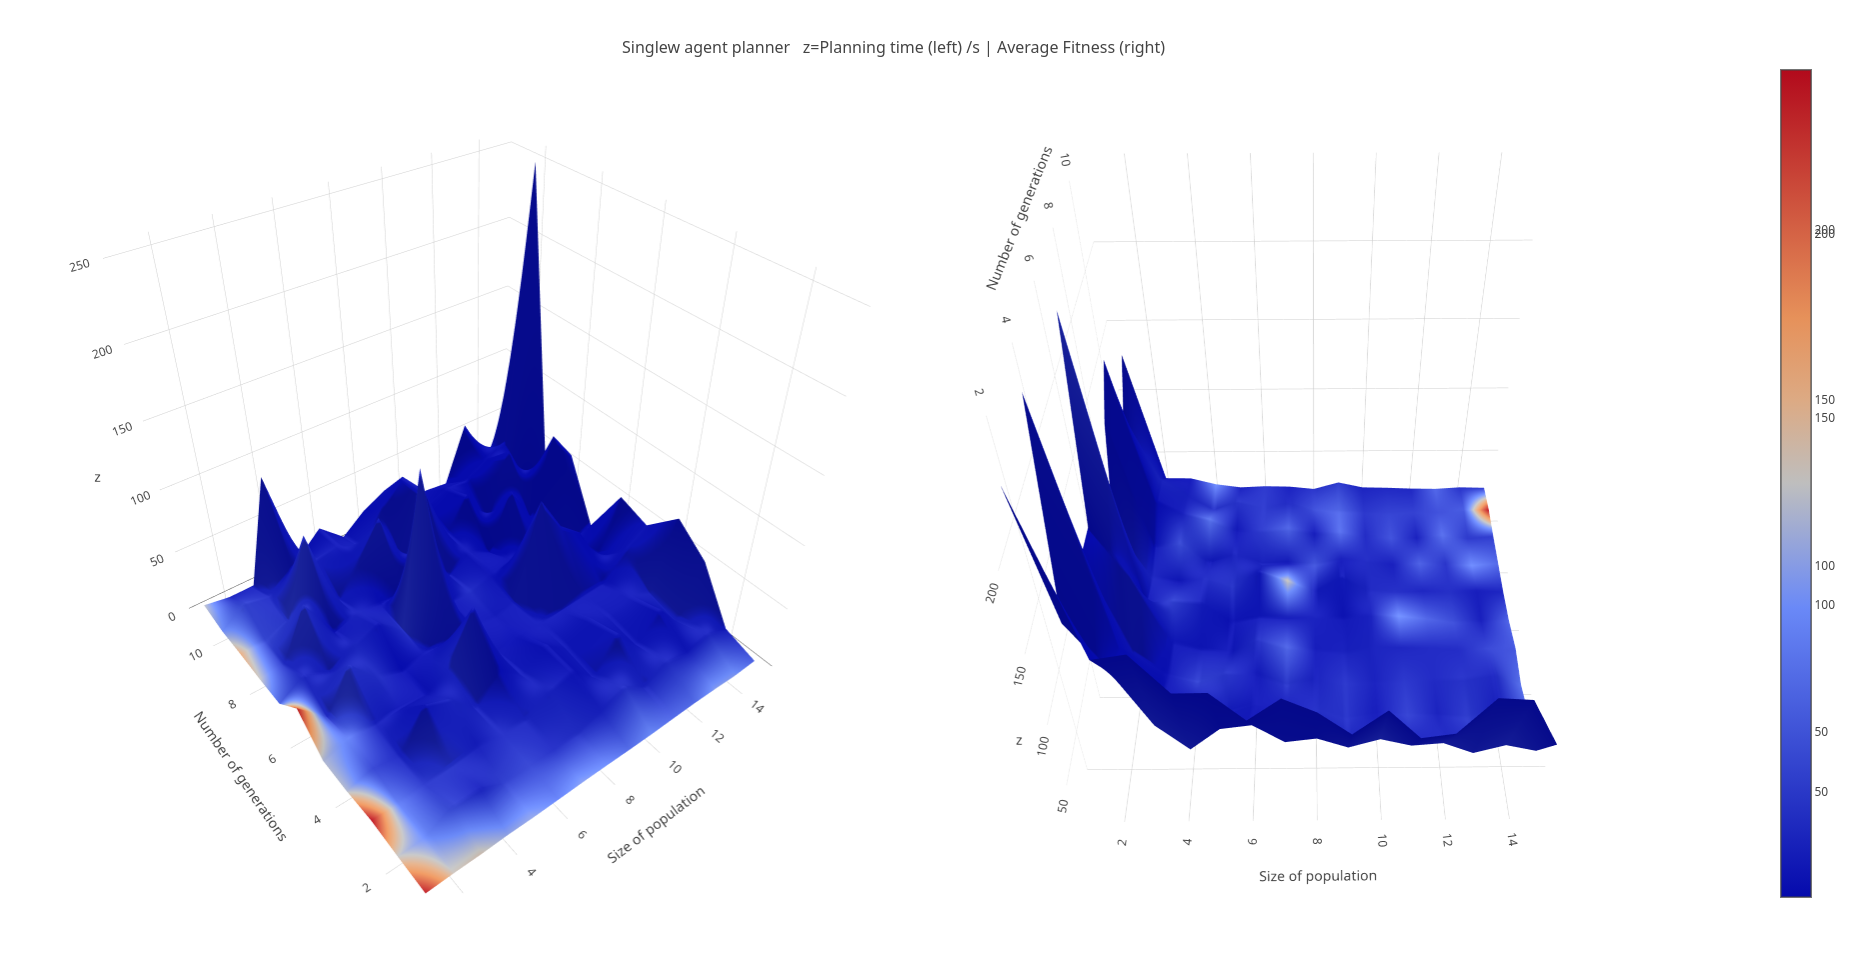
\includegraphics[scale=0.2]{figures/sa-diff3.png}
  \caption{\label{fig:sa-diff3} Single agent planning: number of generations against size of population against planning time (left) /s, fitness (right), over \textit{difficult} road space (Figure~\ref{subfig:sa-road3})}
\end{figure}

\begin{figure}[ht]
  \centering
  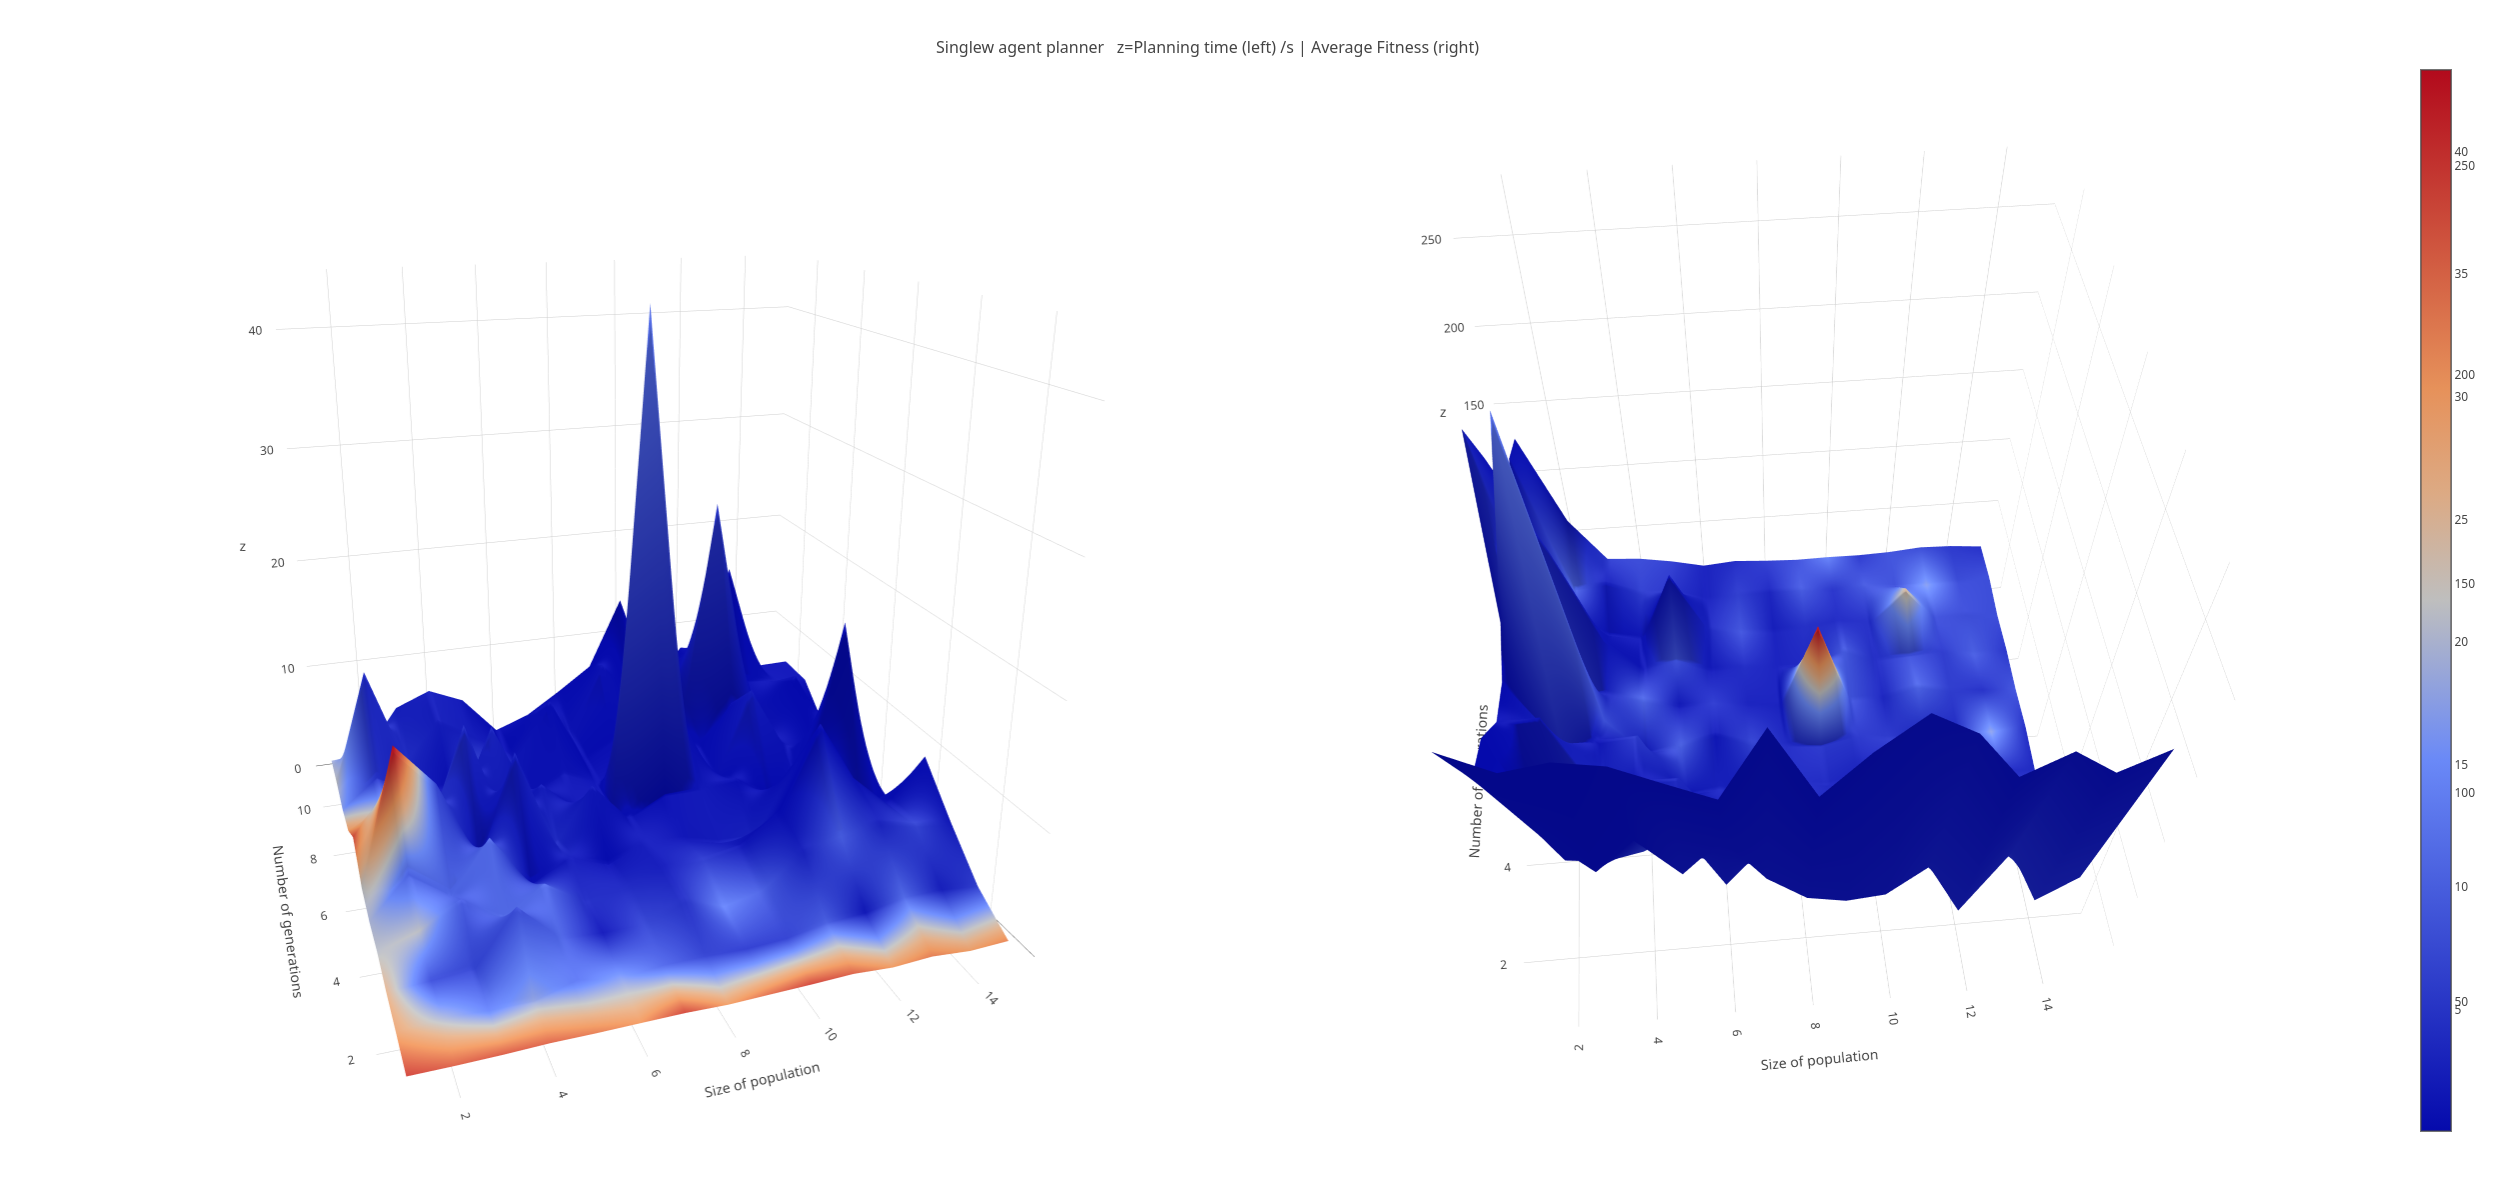
\includegraphics[scale=0.15]{figures/sa-diff4.png}
  \caption{\label{fig:sa-diff4} Single agent planning: number of generations against size of population against planning time (left) /s, fitness (right), over \textit{difficult} road space (Figure~\ref{subfig:sa-road4})}
\end{figure}

\begin{figure}
  \centering
  \begin{subfigure}[b]{0.44\textwidth}
    \centering
    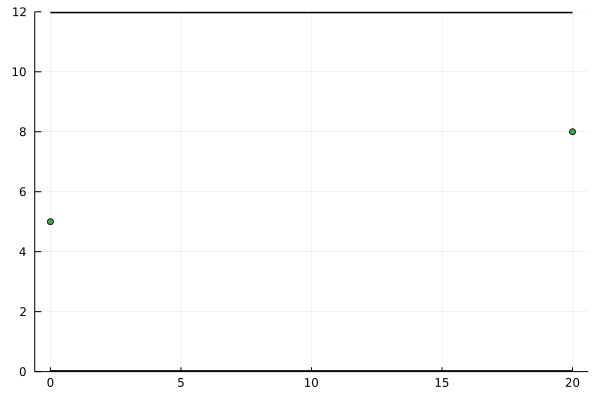
\includegraphics[width=\textwidth]{figures/sa-road1.png}
    \caption{\label{subfig:sa-road1}Easiest road segment, no obstacles, straight}
  \end{subfigure}
  \begin{subfigure}[b]{0.44\textwidth}
    \centering
    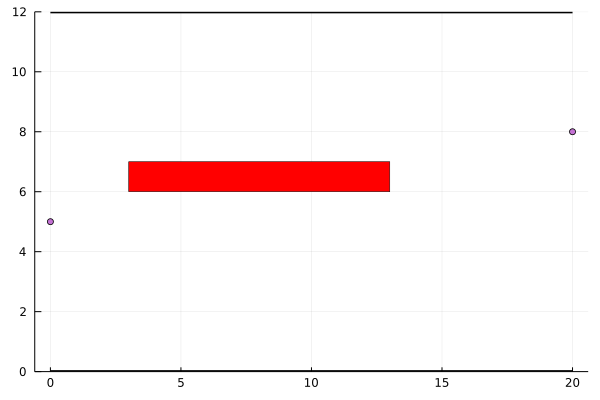
\includegraphics[width=\textwidth]{figures/sa-road2.png}
    \caption{\label{subfig:sa-road2}Second easiest road segment, single, small obstacle in a straight road. Approx. 4\% of road is infeasible}
  \end{subfigure}
  \begin{subfigure}[b]{0.44\textwidth}
    \centering
    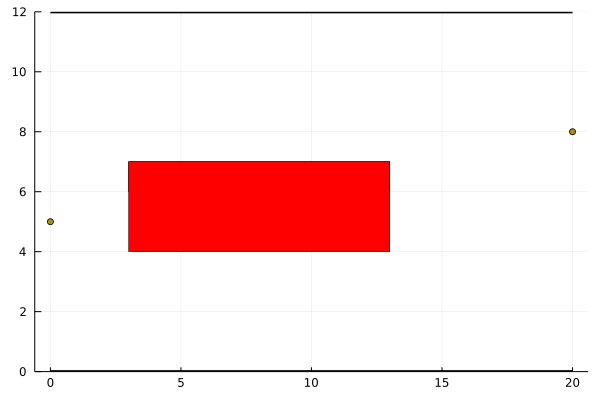
\includegraphics[width=\textwidth]{figures/sa-road3.png}
    \caption{\label{subfig:sa-road3}Road segment with single, large obstacle in a straight road. Approx. 12.5\% of road is infeasible.}
  \end{subfigure}
  \begin{subfigure}[b]{0.44\textwidth}
    \centering
    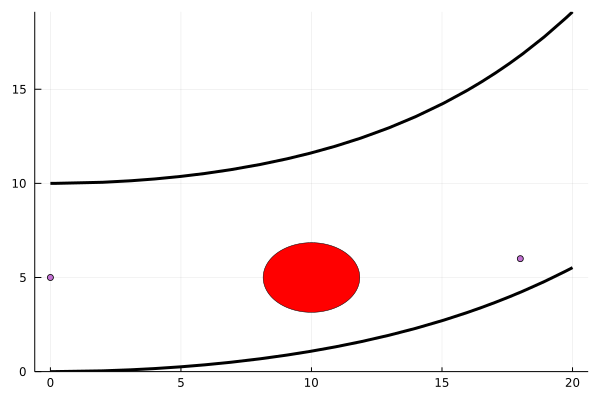
\includegraphics[width=\textwidth]{figures/sa-road4.png}
    \caption{\label{subfig:sa-road4}Road segment with single, medium sized obstacle in a curved road. Approx. 4.9\% of road is infeasible.}
  \end{subfigure}
  \caption{\label{fig:single-agent-roads} Roads used to test single agent planner performance, start and goal positions shown, ordered in terms of difficulty}
\end{figure}

\begin{figure}
  \centering
  \begin{subfigure}[b]{0.44\textwidth}
    \centering
    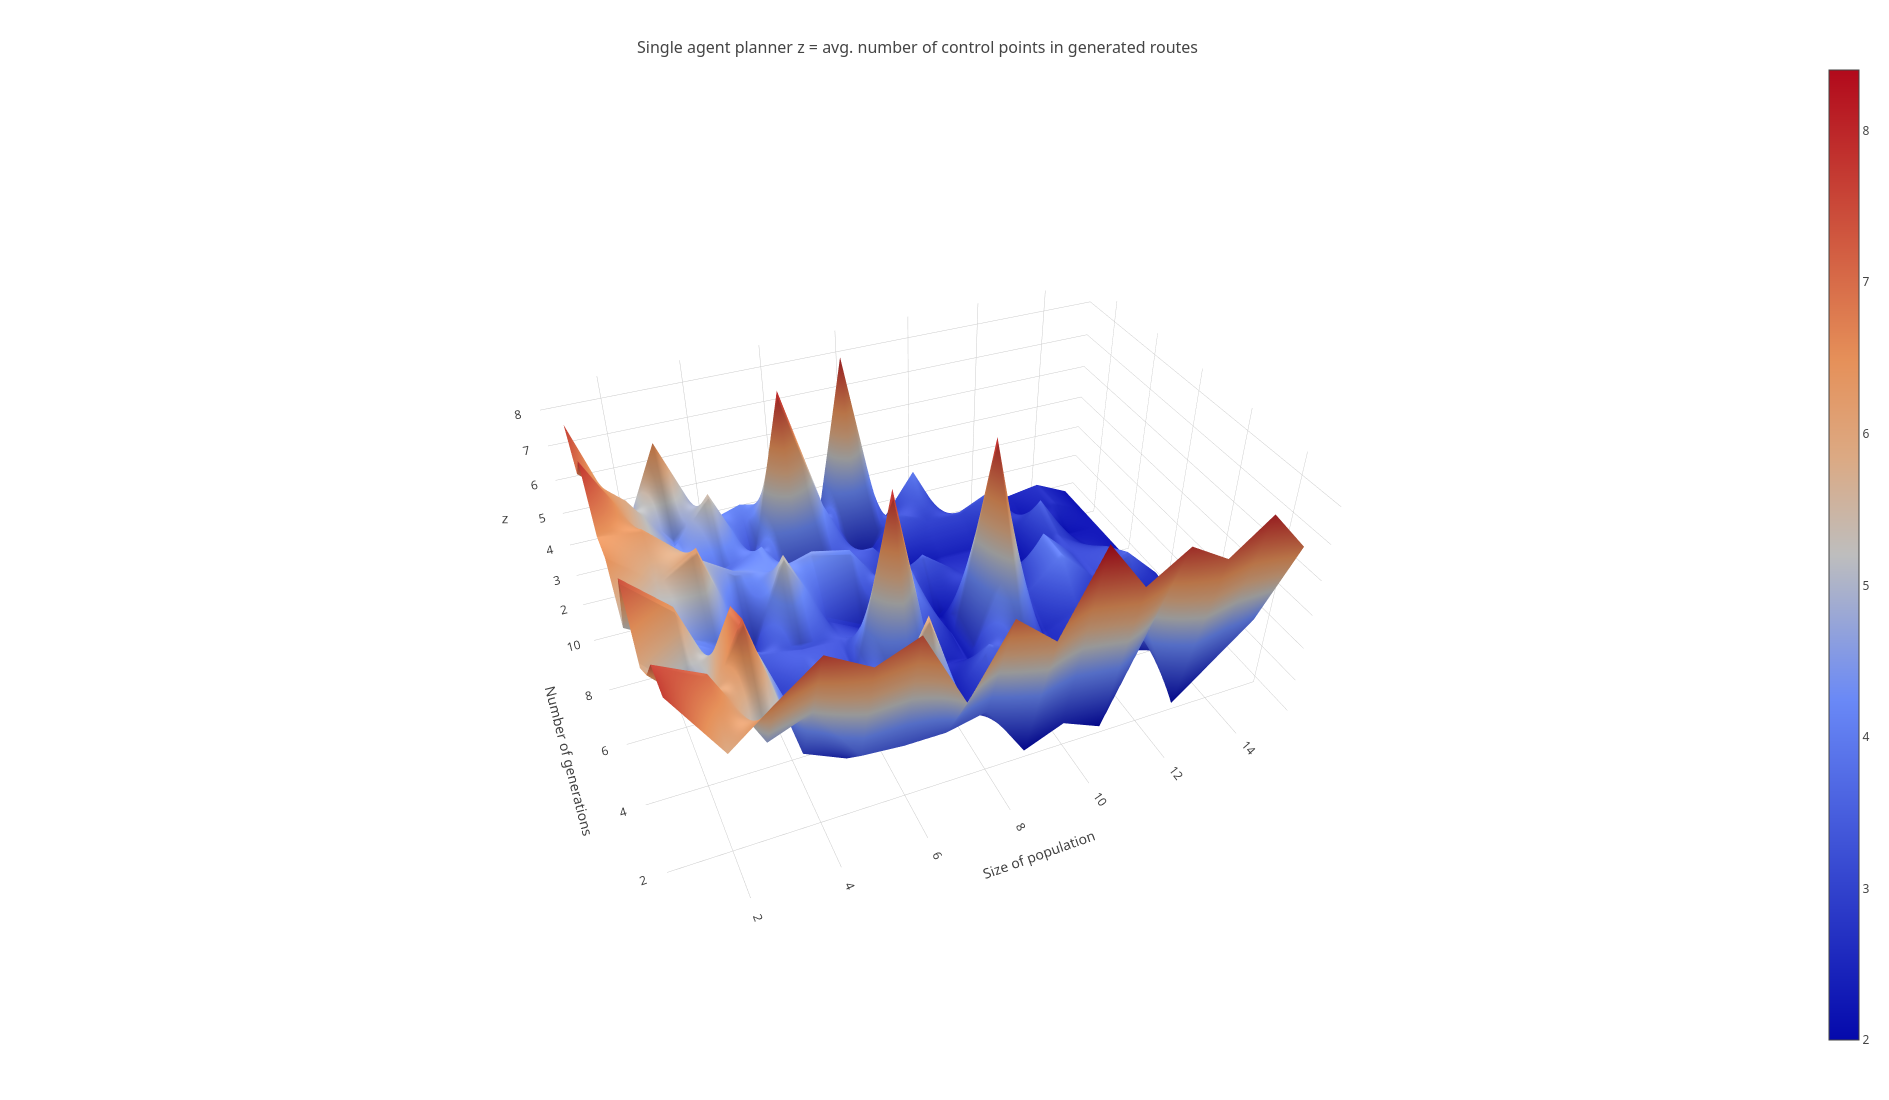
\includegraphics[width=\textwidth]{figures/sa-diff1-cps.png}
    \caption{\label{subfig:sa-diff1-cps}Average number of control points in routes for Road~\ref{subfig:sa-road1}}
  \end{subfigure}
  \begin{subfigure}[b]{0.44\textwidth}
    \centering
    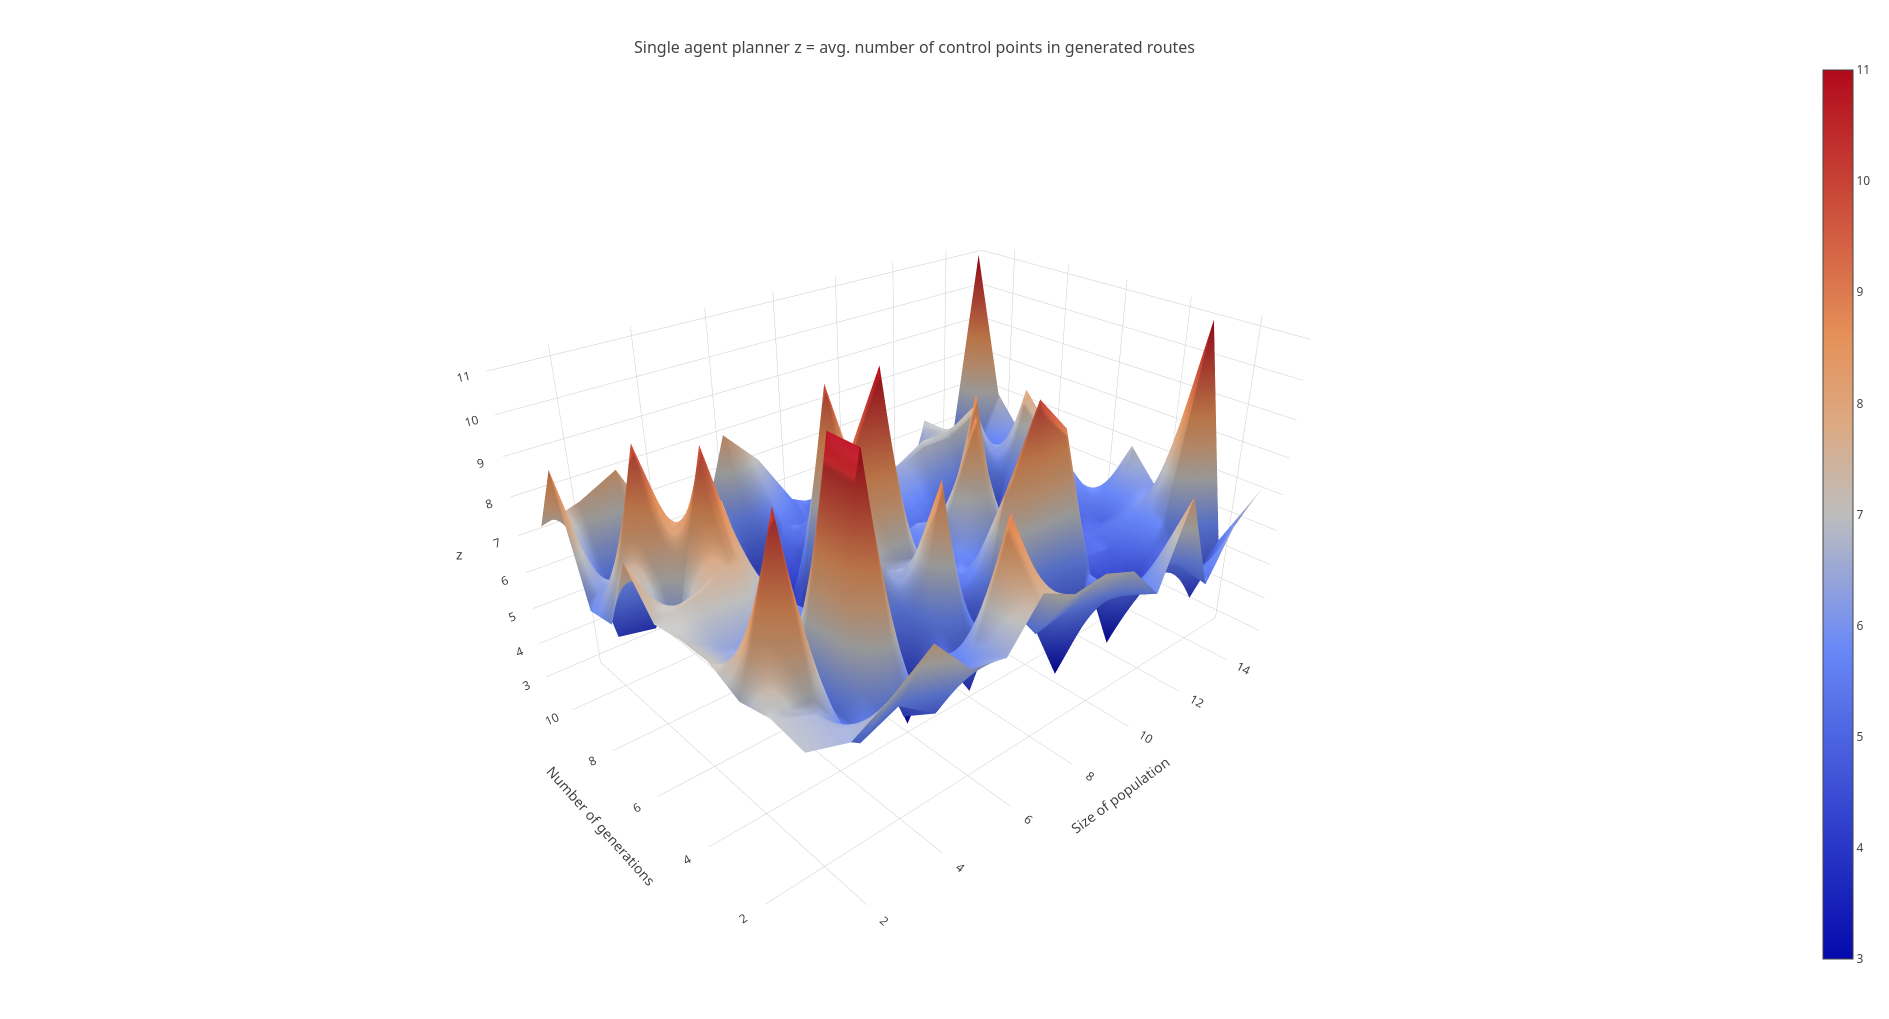
\includegraphics[width=\textwidth]{figures/sa-diff2-cps.png}
    \caption{\label{subfig:sa-diff2-cps}Average number of control points in routes for Road~\ref{subfig:sa-road2}}
  \end{subfigure}
  \begin{subfigure}[b]{0.44\textwidth}
    \centering
    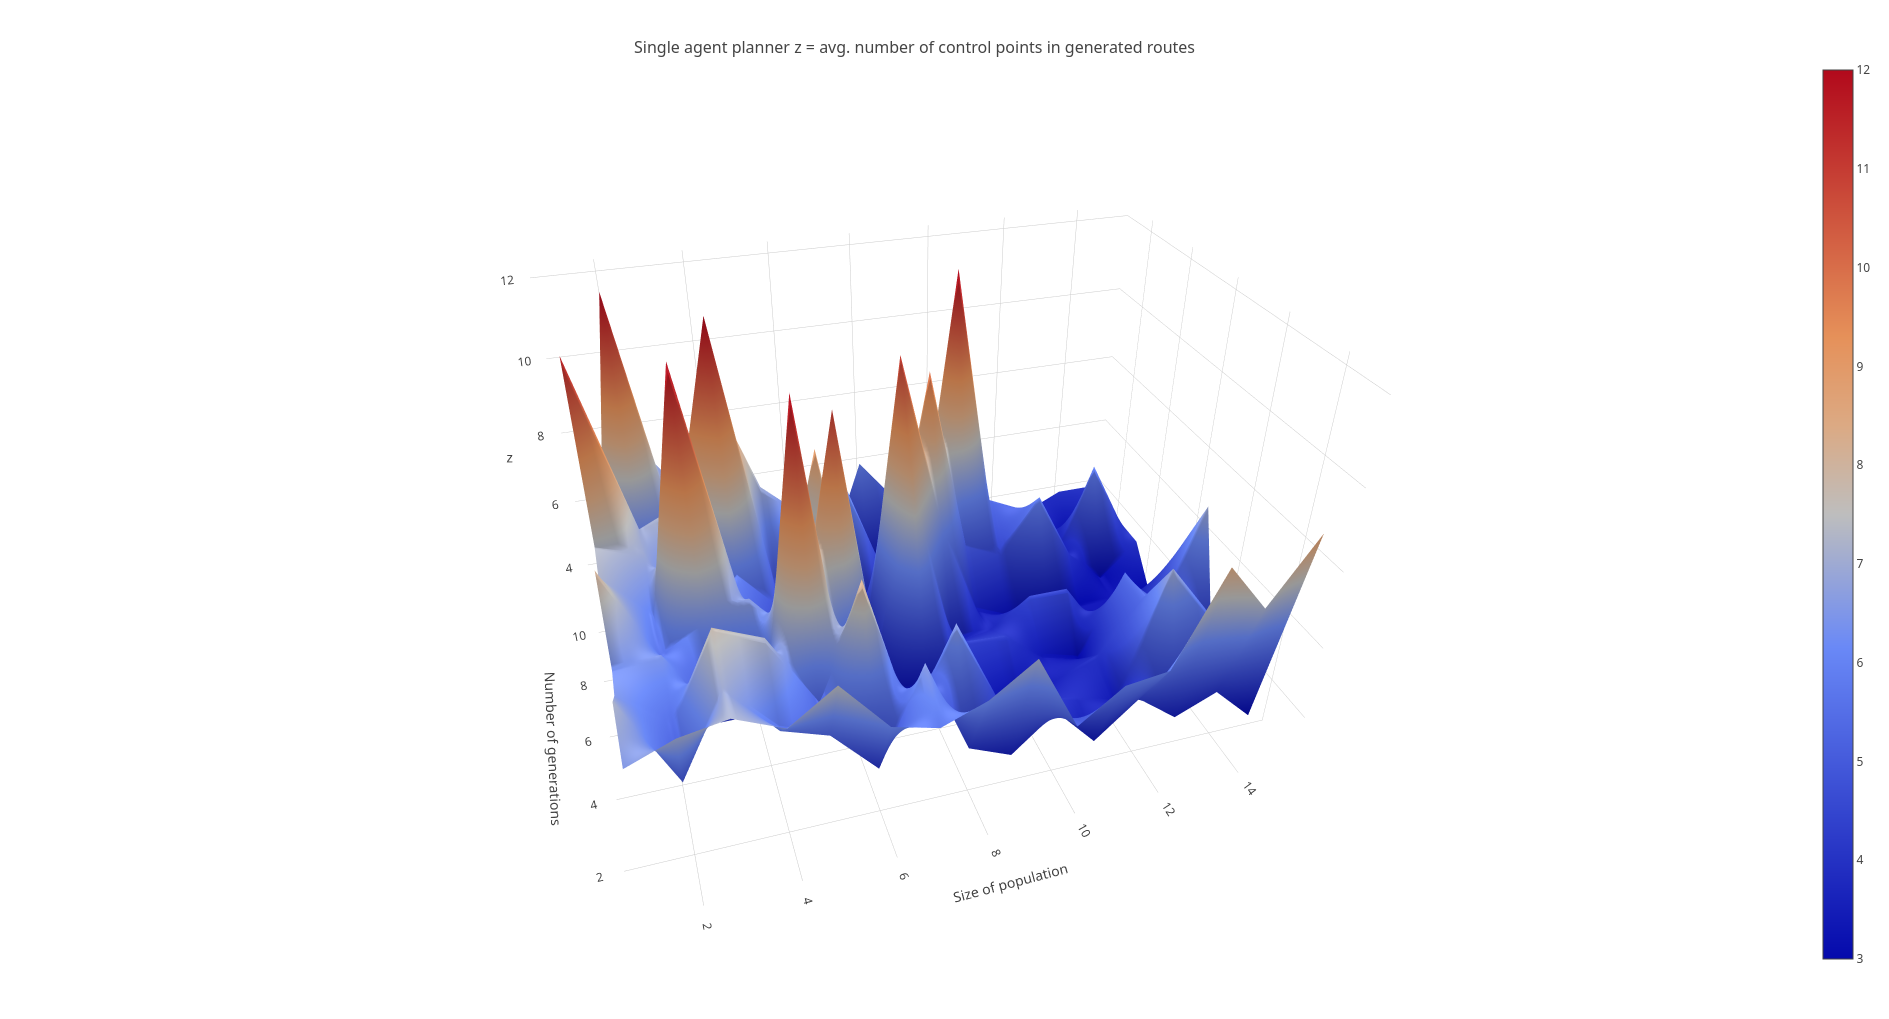
\includegraphics[width=\textwidth]{figures/sa-diff3-cps.png}
    \caption{\label{subfig:sa-diff3-cps}Average number of control points in routes for Road~\ref{subfig:sa-road3}}
  \end{subfigure}
  \begin{subfigure}[b]{0.44\textwidth}
    \centering
    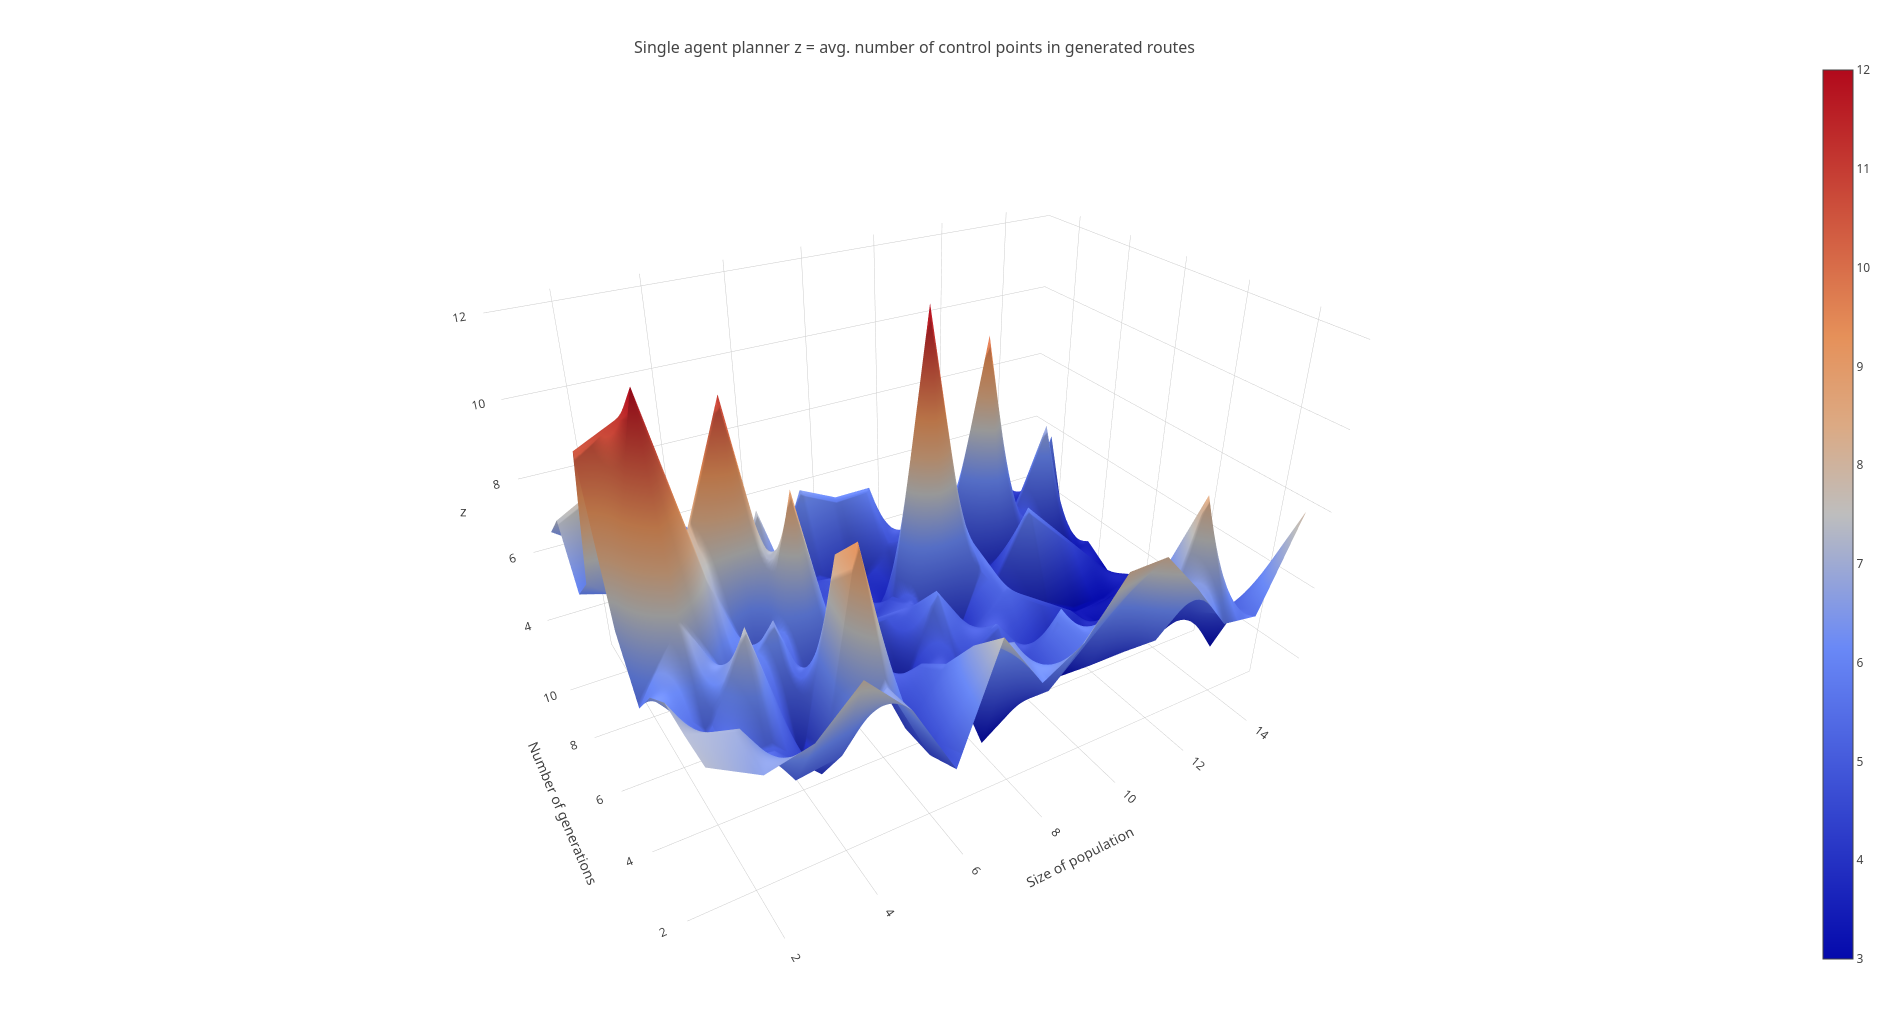
\includegraphics[width=\textwidth]{figures/sa-diff4-cps.png}
    \caption{\label{subfig:sa-diff4-cps}Average number of control points in routes for Road~\ref{subfig:sa-road4}}
  \end{subfigure}
  \caption{\label{fig:single-agent-cps} Average solution complexity for a single agent over a varying number of generations and sizes of populations across various roads }
\end{figure}

\todo{Check units for planning time + add link to hosted dynamic version}

In general, I feel that my single agent planner performs well\footnote{\textbf{Note:} all data used in creating the figures referenced in this section can be found in the \textit{sa-all-data.csv} file included with this report }. In a road space such as the one shown in Figure~\ref{subfig:sa-road1} my algorithm converges to within 10\% of the fitness of a direct line between the start and goal point within 2 generations over 4 individuals as seen in Figure~\ref{fig:sa-col}\footnote{interactive plot can be found \href{https://barrett370.github.io/Y4-Diss/single-agent-result-1404-col}{here}: https://barrett370.github.io/Y4-Diss/single-agent-result-1404-col}.

As the road space complexity increases (See Figures~\ref{subfig:sa-road2},\ref{subfig:sa-road3}), the speed at which my algorithm convergence is reduced.

Over the road space seen in Figure~\ref{subfig:sa-road2}, this is only by a small margin, taking closer to 3 generations (See Figure~\ref{fig:sa-diff2}\footnote{interactive plot can be found \href{https://barrett370.github.io/Y4-Diss/single-agent-result-diff2}{here}: https://barrett370.github.io/Y4-Diss/single-agent-result-diff2}).

However, on a more difficult example such as that seen in Figure~\ref{subfig:sa-road3}, all routes close to a straight line are infeasible, resulting in a lower average fitness as can be seen in Figure~\ref{fig:sa-diff3}\footnote{interactive plot can be found \href{https://barrett370.github.io/Y4-Diss/single-agent-result-diff3}{here}: https://barrett370.github.io/Y4-Diss/single-agent-result-diff3}, as well as a higher average planning time as it is required to perform more involved infeasible distance calculations more often.

On the example road shown in Figure~\ref{subfig:sa-road4}, the algorithm converges slower still, but still reaching what I would consider to be a \textit{good} solution within 5 generations with a population size around 7, these results can be seen in Figure~\ref{fig:sa-diff4}\footnote{interactive plot can be found, Link points here:}\todo{update this footnote}. In terms of planning time, with a few anomalous exceptions planning time steadily increases roughly proportionally to (the number of generations $\times$ the population size).

In general, the analysis of the planning time for my algorithm is difficult due to the inherent stochastic nature of Genetic algorithms. As such, you may notice many erroneous spikes in seemingly random places across the results surfaces, however, in all cases a general upward trend in planning time is seen.\todo{move this to end of evaluation?}

\section{Cooperative (Multi-agent) Planning}
\label{subsec:eval-cooperativeplanning}

My solution to the problem of planning $n$ non-colliding routes for $n$ agents was so wrap my existing \texttt{GA} function in a cooperative \textit{layer}. This cooperative layer relied on a function for detecting collisions which had extremely high overhead, at one point causing around 50x slowdown in the running time of the function. Detecting intersections between two Bézier curves is a non-trivial task with the best methods taking the same approach of recursive subdivision that I utilised.

As detailed in Section~\ref{sec:maa}, I attempted to speedup my cooperative planning layer through many different means, including parallelising the entire method as well as individual high-complexity sections such as the Bézier curve intersection function. The system on which I have been benchmarking performance is equipped with 16 cores running at a maximum of 4.2GHz.

Julia boasts the ability to distribute work across multiple systems over secure shell, this could conceivably allow for on-board vehicle computers to aid in the computation and planning of their own routes. Each individual in a concurrent plan is spawned as a unique threaded task and as such having cores equal to the number of concurrently planned agents is ideal. Julia also has good support for GPU programming through libraries such as \texttt{CUDA.jl}\cite{besard2018juliagpu}, in their 2018 paper Roberge et al.\cite{robergeFastGeneticAlgorithm2018} showed how effective massively parallelising genetic algorithms can be, seeing a 290x speedup when compared to sequential execution on a CPU.\@ These two factors make the relatively high planning times seen in this report potentially immaterial and could allow for much higher numbers of generations or larger populations to be feasible.\todo{move this para?}

I tested my cooperative planning method against the same road sections I used to test the single agent planner and unless stated otherwise tested with 3 agents with start-goal positions seen in Figure~\ref{fig:multi-agent-roads}. In all cases I used Gaussian mutation, ranked selection and simple crossover.

When considering the easiest road section, Figure~\ref{subfig:ma-road1}, the average fitness of individuals at low generations and population size is incredibly high, leading to me thresholding it at 40 when producing Figure~\ref{fig:ma-diff1-lim40}. However, it quickly drops producing \textit{good} solutions with average fitness in the region of 18 to 20 within 4 generations over populations around 5 in size.

Planning time sees typical steady growth as the number of generations and population size increases, peaking at around 1 minute (excluding anomalous results) but averaging closer to 40 seconds at the higher end of population size and generations.

\begin{figure}[ht]
  \centering
  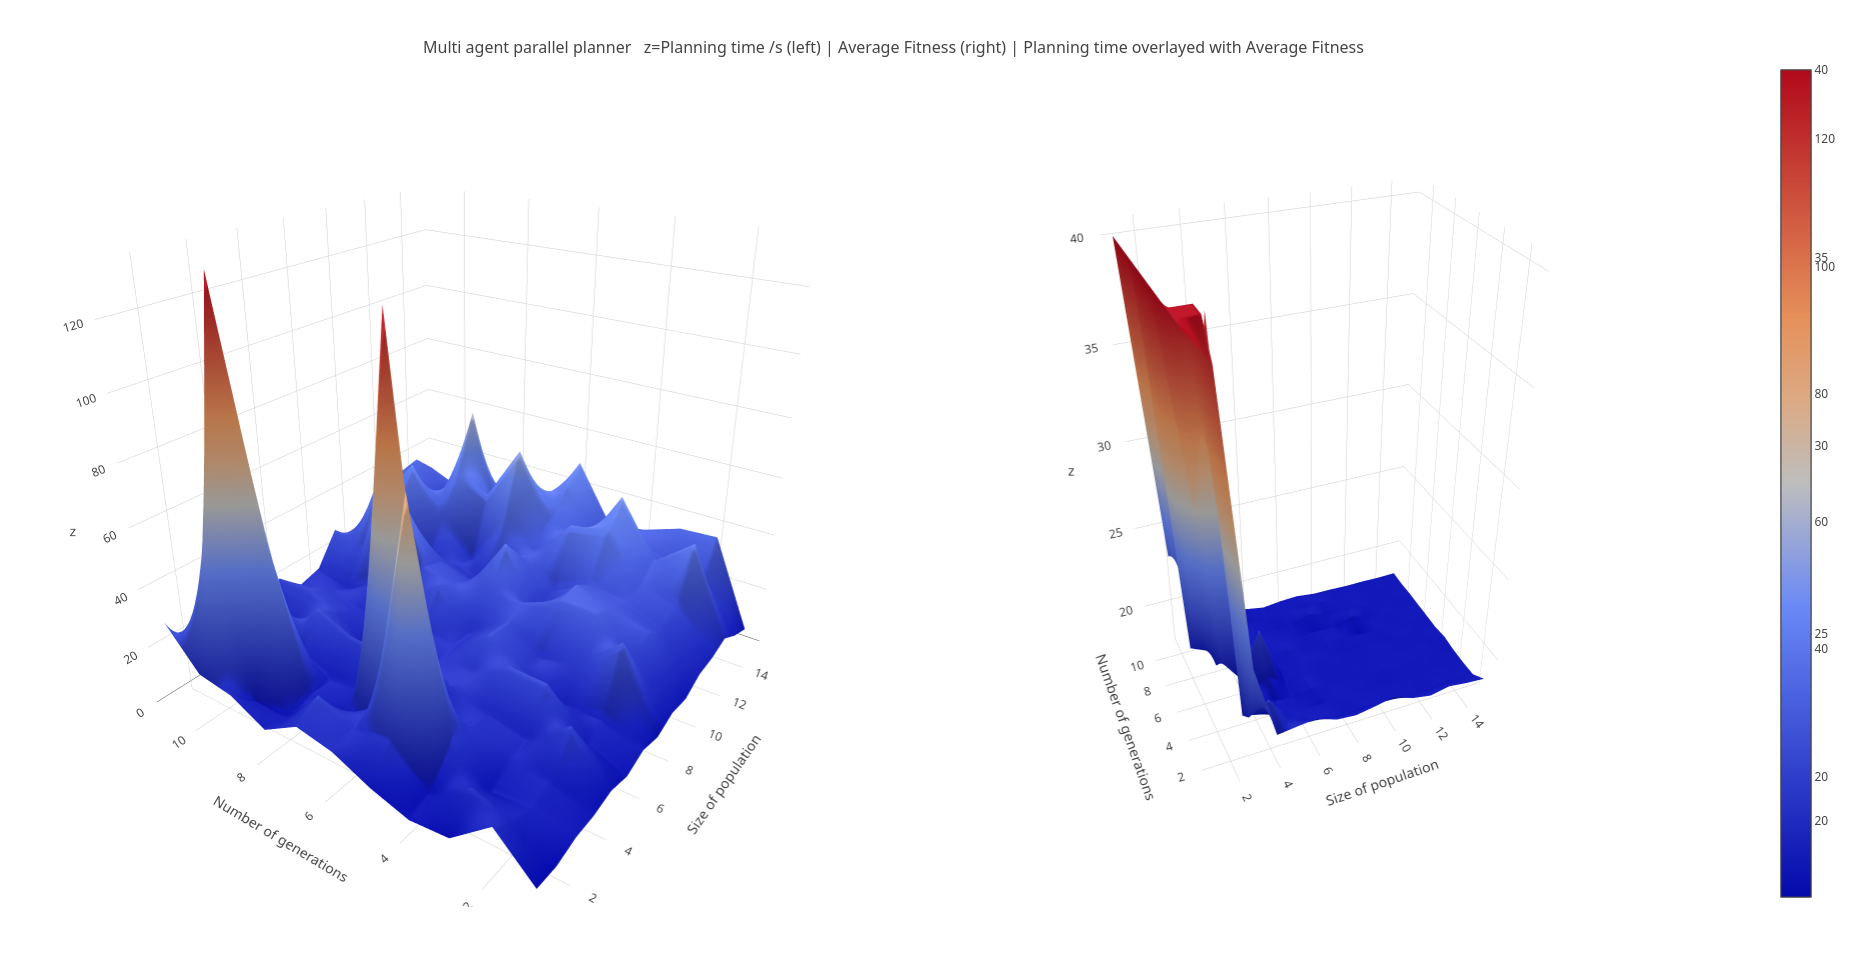
\includegraphics[scale=0.19]{figures/ma-diff1.png}
  \caption{\label{fig:ma-diff1-lim40} Multi agent planning number of generations against size of population against planning time (left), fitness limited at 40 (right), planning through road seen in Figure~\ref{subfig:ma-road1}}
\end{figure}

On a road with an obstacle (Figure~\ref{subfig:ma-road2}), the result seen in Figure~\ref{fig:ma-diff2-lim40} is achieved. Taking slightly longer to converge to \textit{good} solutions at around 6 generations over 6 population. It appears that the number of generations has more of an effect on fitness with 6 generations over 5 populations showing better results than 4 generations on 7 population. However planning time appears to suffer more from more generations than it does from larger populations.

\begin{figure}[ht]
  \centering
  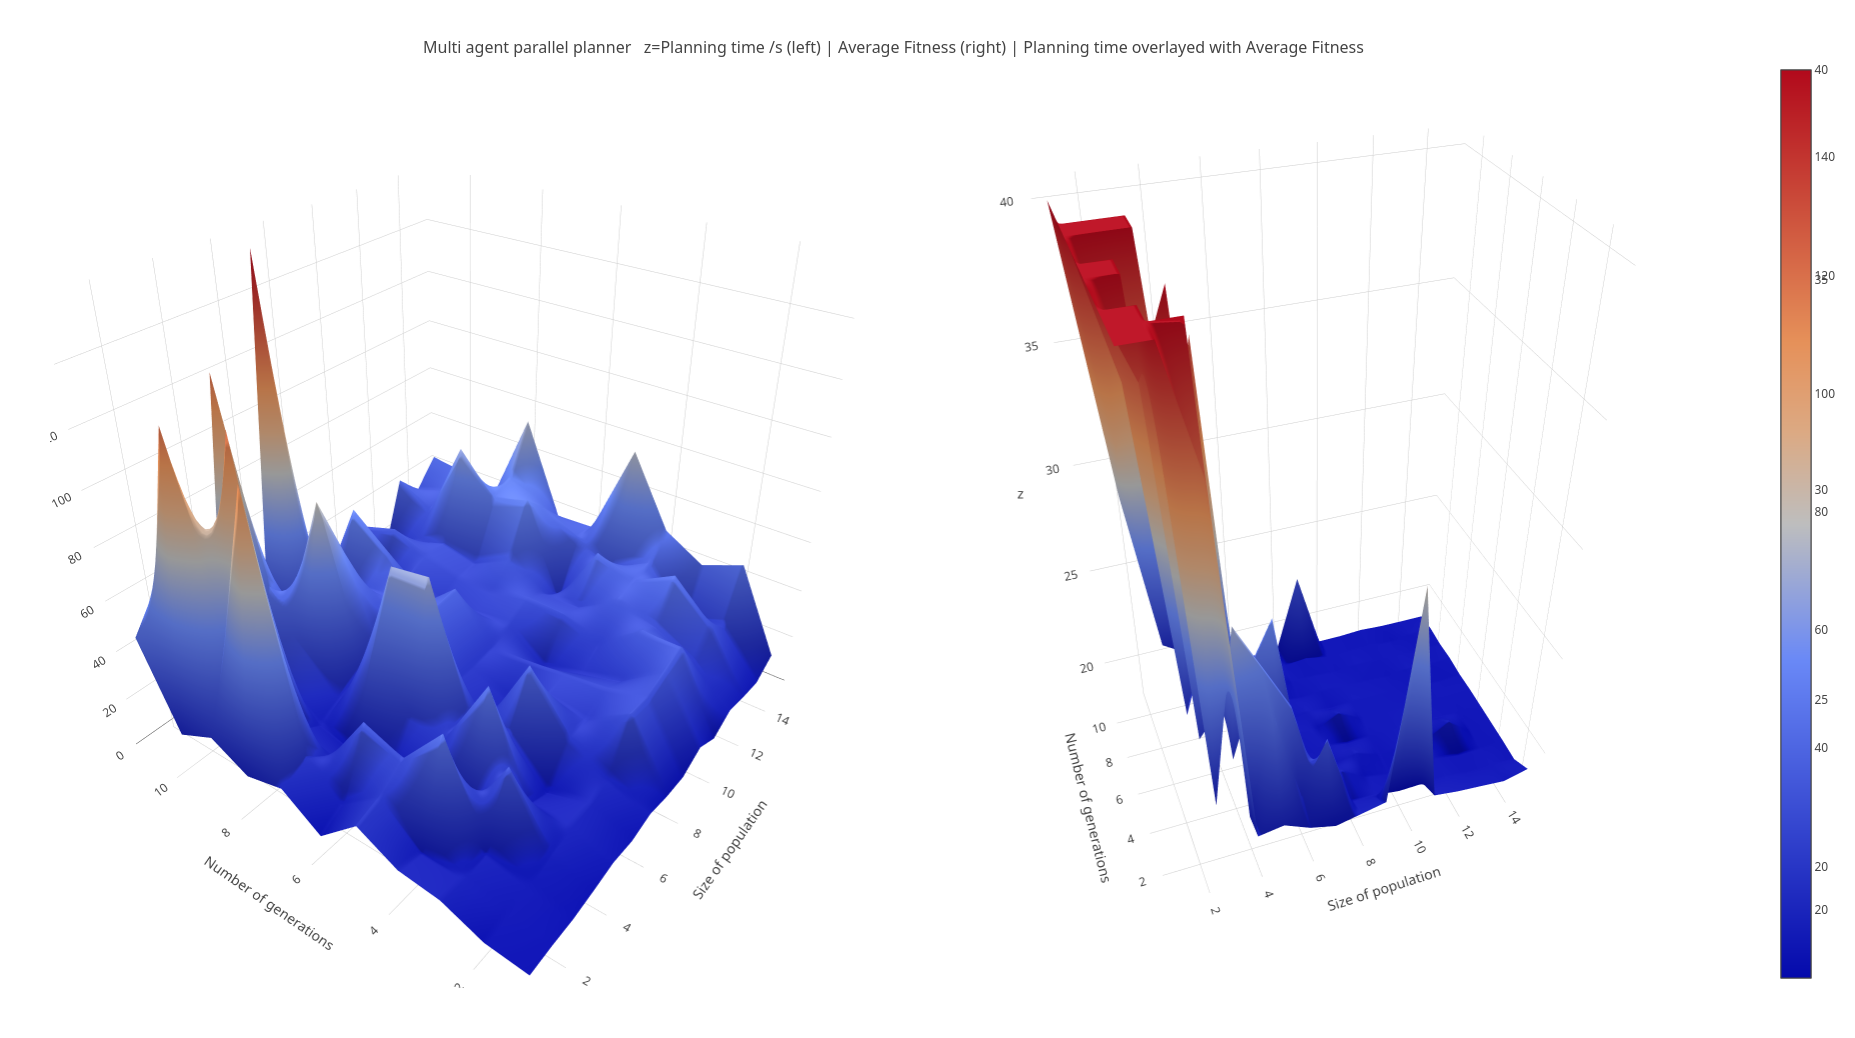
\includegraphics[scale=0.19]{figures/ma-diff2.png}
  \caption{\label{fig:ma-diff2-lim40} Multi agent planning number of generations against size of population against planning time (left), fitness limited at 40 (right), planning through road seen in Figure~\ref{subfig:ma-road2}}
\end{figure}


Increasing the difficulty further, over the road seen in Figure~\ref{subfig:ma-road3}, we see a yet slower convergence rate with consistently \textit{good} results appearing after 8 generations over 8 individuals, we do however see the fitness drop steeply between the 7th and 8th generations, much more steeply than in the \textit{easier} road segments. Planning time is significantly higher than in previous tests with an average planning rising to around 3 minutes on high numbers of generations and sizes of populations.

\begin{figure}[ht]
  \centering
  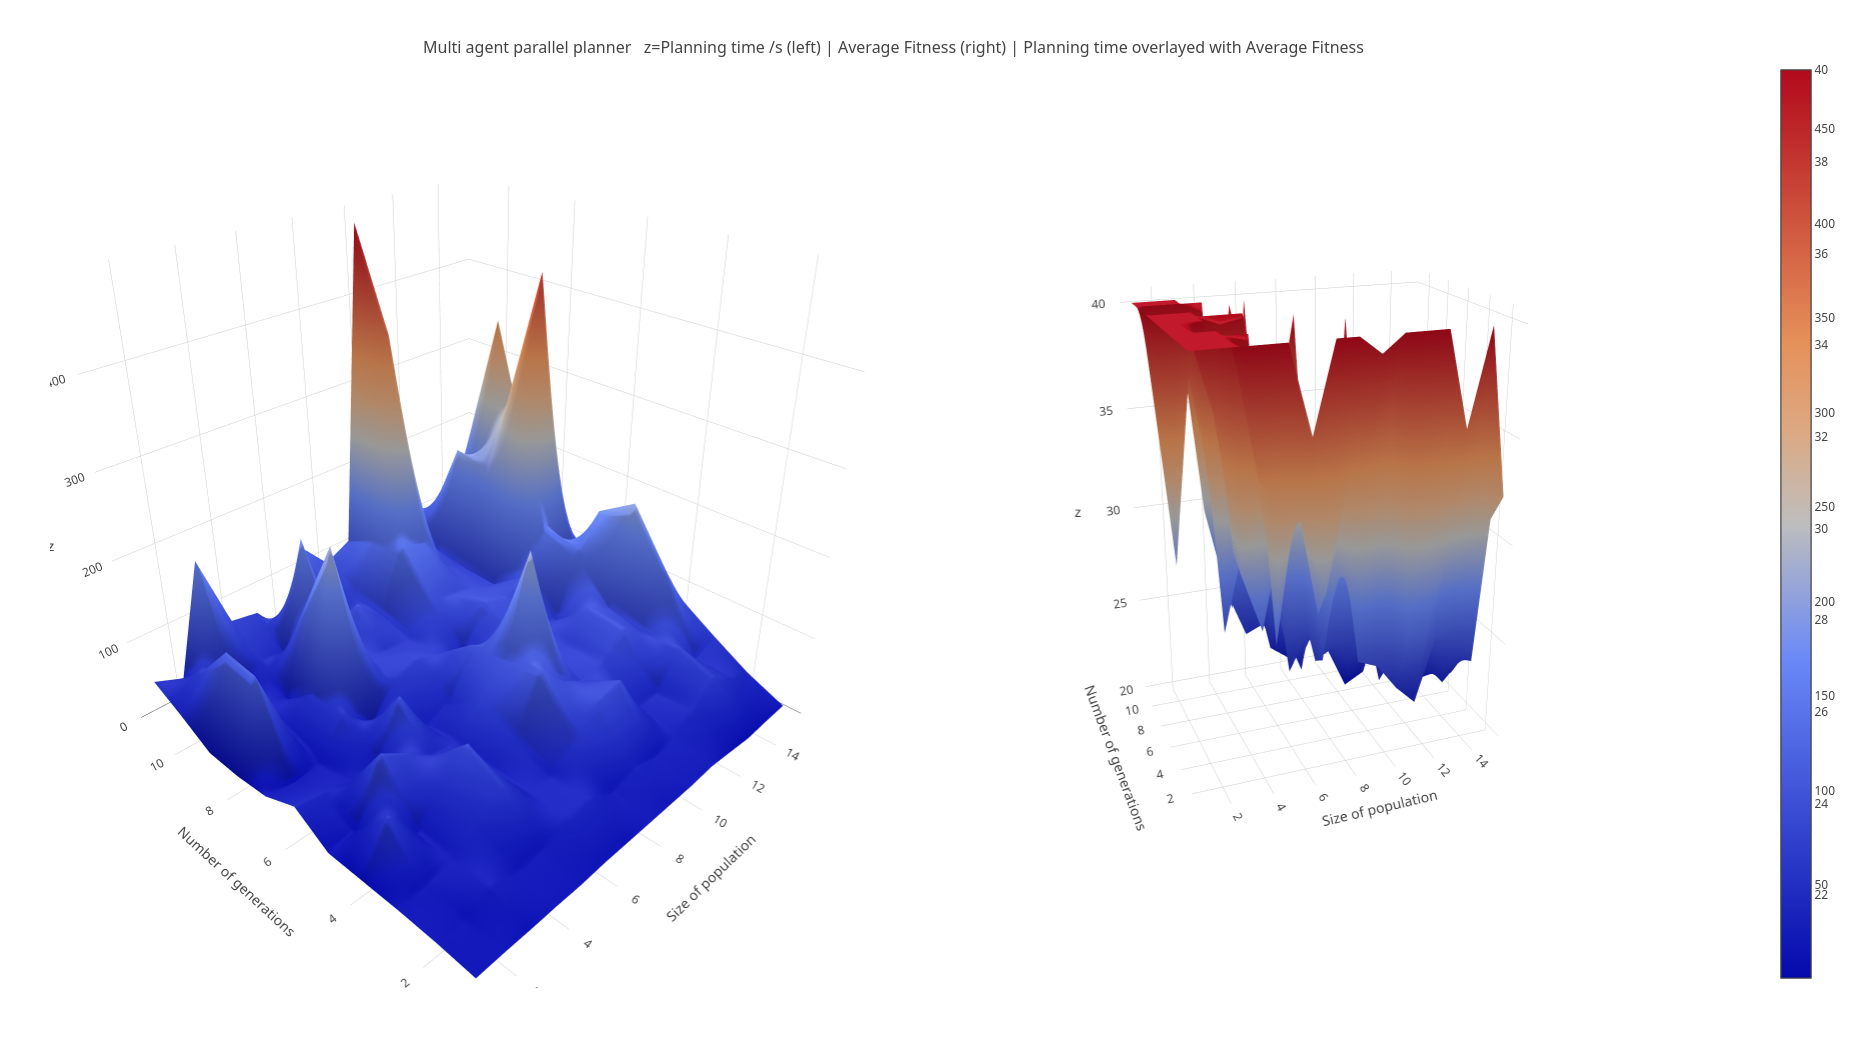
\includegraphics[scale=0.19]{figures/ma-diff3.png}
  \caption{\label{fig:ma-diff3-lim40} Multi agent planning number of generations against size of population against planning time (left), fitness limited at 40 (right), planning through road seen in Figure~\ref{subfig:ma-road3}}
\end{figure}


When planning on the most difficult road segment (Figure~\ref{subfig:ma-road4}), my approach appears to be much less stable. In Figure~\ref{fig:ma-diff4}, you can clearly see the fitness still peaks above 200 regularly even after a high number of generation and/or population size. Whilst a general trend lower fitness can be seen, the regular spikes mean collisions or intersections with the obstacle are common, producing infeasible routes. Clearly more work is required for my approach to handle these more complex road spaces well, as well as perhaps higher populations / numbers of generations.

Planning time again is seen to trend upwards proportionally with (number of generations $\times$ size of populations), reaching very high planning times peaking at 280 seconds for 10 generations over populations of size 15 although, interestingly this is lower than the times seen when planning for Figure~\ref{subfig:ma-road3}, this may be due to the start and goal positions changing leading to more routes in which collision detection can be exited early, i.e. routes in which intersections occur early in the trajectory. This could also be due to external factors such as increased background load on my system during the planning of Road~\ref{subfig:ma-road3}

When varying the number of agents being concurrently planned for we can see that the planning time steadily increases with each new agent added. In Figure~\ref{fig:ma-vary-a} where the planning time surfaces of runs using 1,2,3 and 4 different agents through the road seen in Figure~\ref{subfig:sa-road1}, the surfaces are shown to layer in order of number of agents, thi


\begin{figure}[ht]
  \centering
  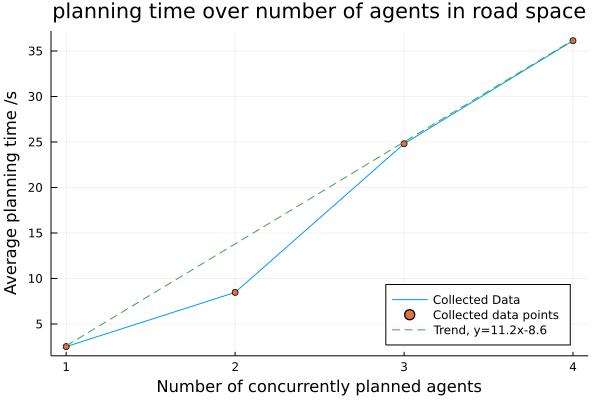
\includegraphics[scale=0.5]{figures/ma-vary-a.png}
  \caption{\label{fig:ma-vary-a} Varying number of agents being concurrently planned through Road~\ref{subfig:ma-road1}}
\end{figure}

\begin{figure}[ht]
  \centering
  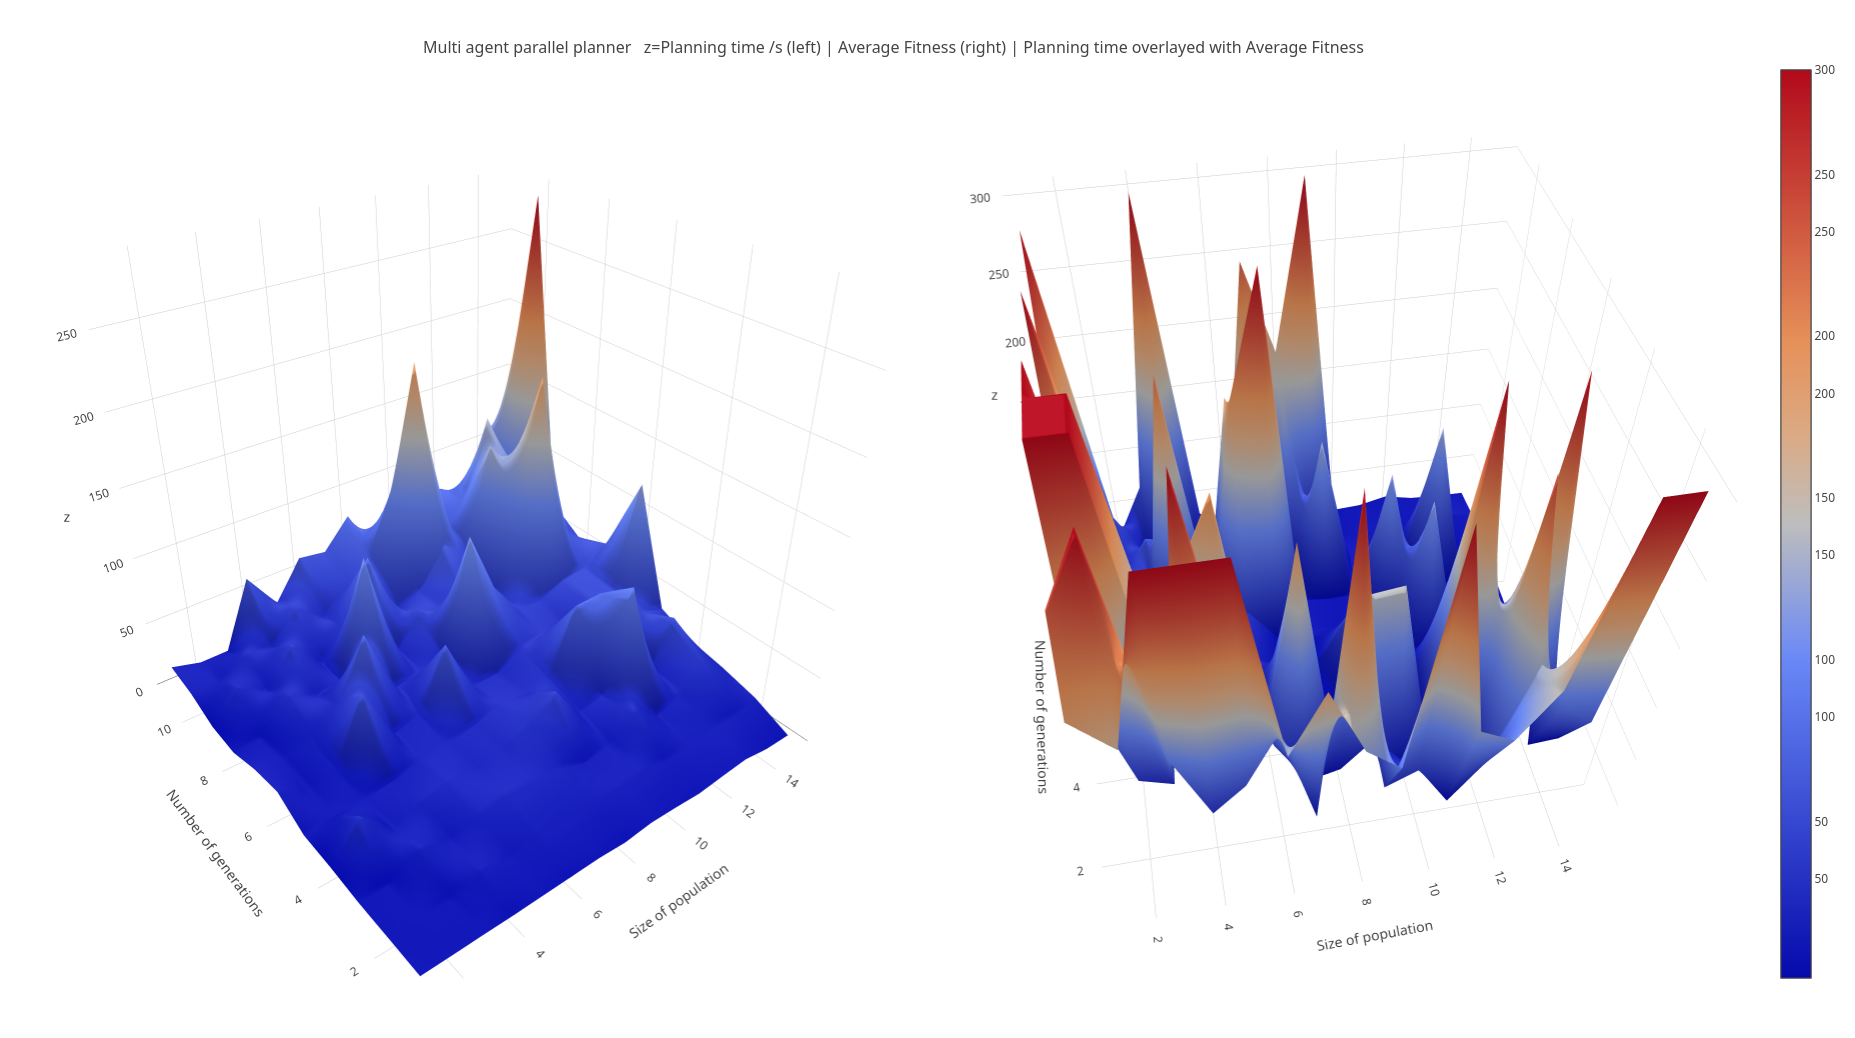
\includegraphics[scale=0.19]{figures/ma-diff4.png}
  \caption{\label{fig:ma-diff4} Multi agent planning number of generations against size of population against planning time (left), fitness limited at 300 (right), planning through road seen in Figure~\ref{subfig:ma-road4}}
\end{figure}

\begin{figure}
  \centering
  \begin{subfigure}[b]{0.44\textwidth}
    \centering
    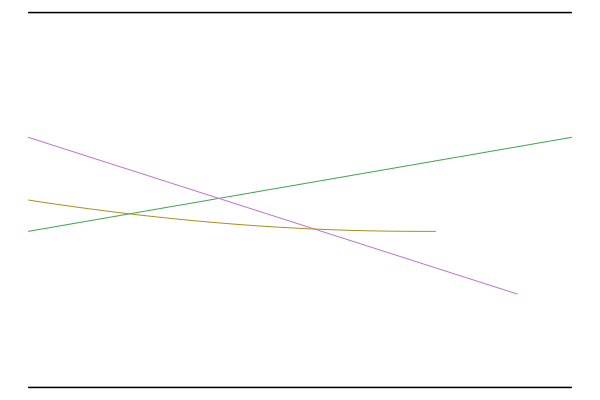
\includegraphics[width=\textwidth]{figures/ma-road1-eg.png}
    \caption{\label{subfig:ma-road1-eg}Example routes through easy road space, average fitness = 18.0 }
  \end{subfigure}
  \begin{subfigure}[b]{0.44\textwidth}
    \centering
    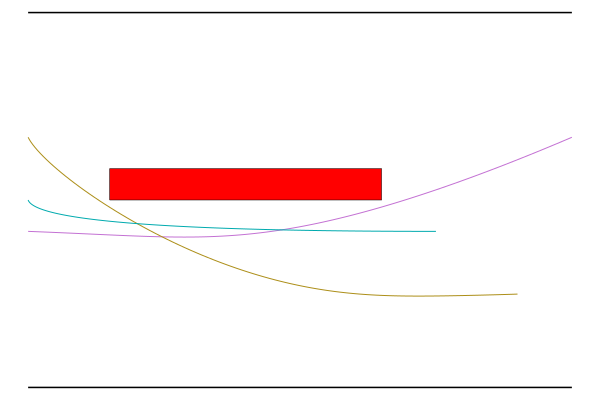
\includegraphics[width=\textwidth]{figures/ma-road2-eg.png}
    \caption{\label{subfig:ma-road2-eg}Example routes through medium road space, average fitness = 18.4 }
  \end{subfigure}
  \begin{subfigure}[b]{0.44\textwidth}
    \centering
    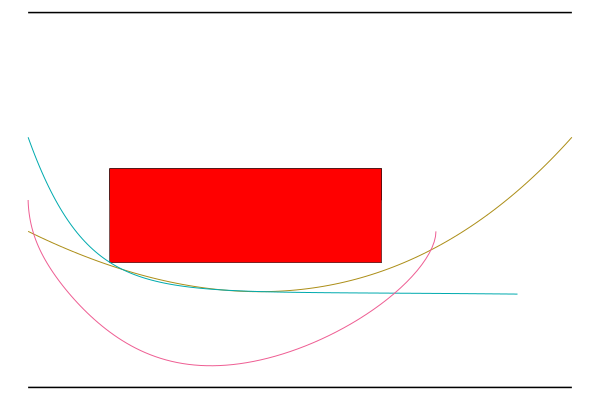
\includegraphics[width=\textwidth]{figures/ma-road3-eg.png}
    \caption{\label{subfig:ma-road3-eg}Example routes through hard road space, average fitness = 155.8}
  \end{subfigure}
  \begin{subfigure}[b]{0.44\textwidth}
    \centering
    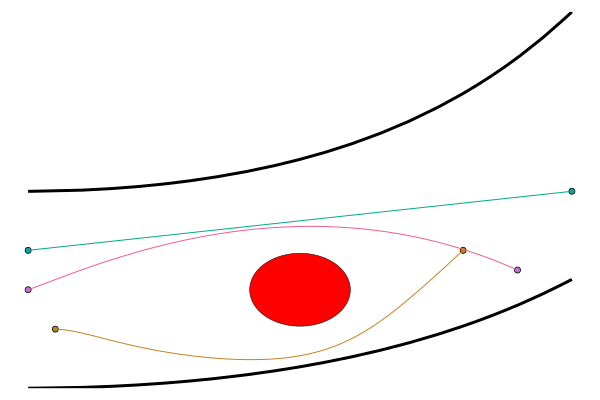
\includegraphics[width=\textwidth]{figures/ma-road4-eg.png}
    \caption{\label{subfig:ma-road4-eg}Example routes through hard, curved road space, average fitness = 19.3 }
  \end{subfigure}
  \caption{\label{fig:multi-agent-roads-egs} Roads used to test single agent planner performance, start and goal positions shown, ordered in terms of difficulty}
\end{figure}


\begin{figure}
  \centering
  \begin{subfigure}[b]{0.44\textwidth}
    \centering
    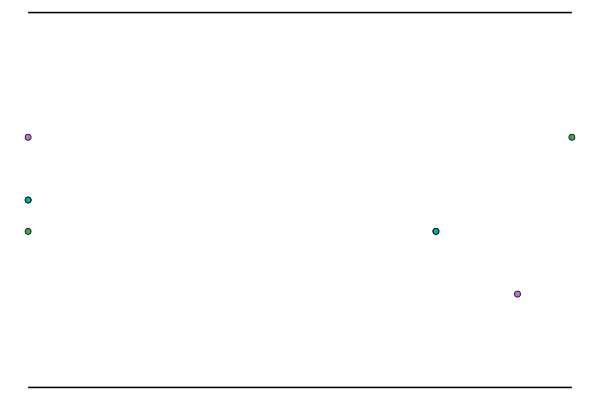
\includegraphics[width=\textwidth]{figures/ma-road1.png}
    \caption{\label{subfig:ma-road1}Easiest road segment, no obstacles, straight}
  \end{subfigure}
  \begin{subfigure}[b]{0.44\textwidth}
    \centering
    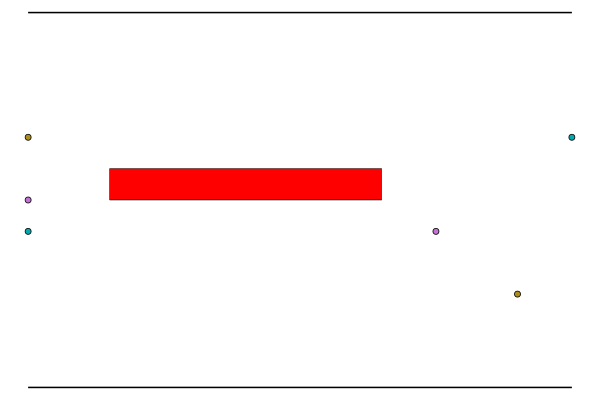
\includegraphics[width=\textwidth]{figures/ma-road2.png}
    \caption{\label{subfig:ma-road2}Second easiest road segment, single, small obstacle in a straight road. Approx. 4\% of road is infeasible}
  \end{subfigure}
  \begin{subfigure}[b]{0.44\textwidth}
    \centering
    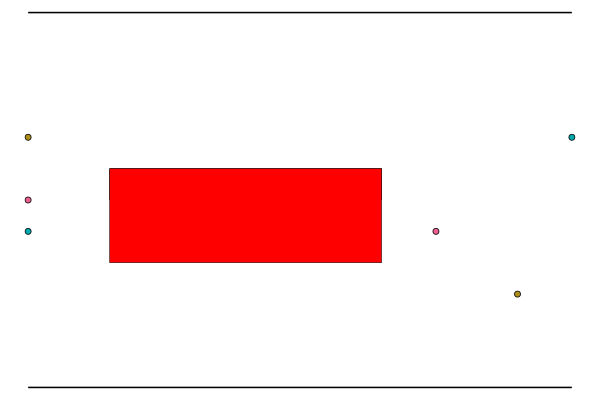
\includegraphics[width=\textwidth]{figures/ma-road3.png}
    \caption{\label{subfig:ma-road3}Road segment with single, large obstacle in a straight road. Approx. 12.5\% of road is infeasible.}
  \end{subfigure}
  \begin{subfigure}[b]{0.44\textwidth}
    \centering
    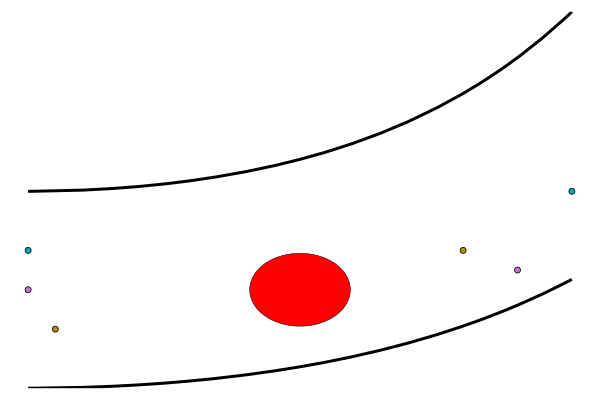
\includegraphics[width=\textwidth]{figures/ma-road4.png}
    \caption{\label{subfig:ma-road4}Road segment with single, medium sized obstacle in a curved road. Approx. 4.9\% of road is infeasible.}
  \end{subfigure}
  \caption{\label{fig:multi-agent-roads} Roads used to test single agent planner performance, start and goal positions shown, ordered in terms of difficulty}
\end{figure}

\begin{figure}
  \centering
  \begin{subfigure}[b]{0.44\textwidth}
    \centering
    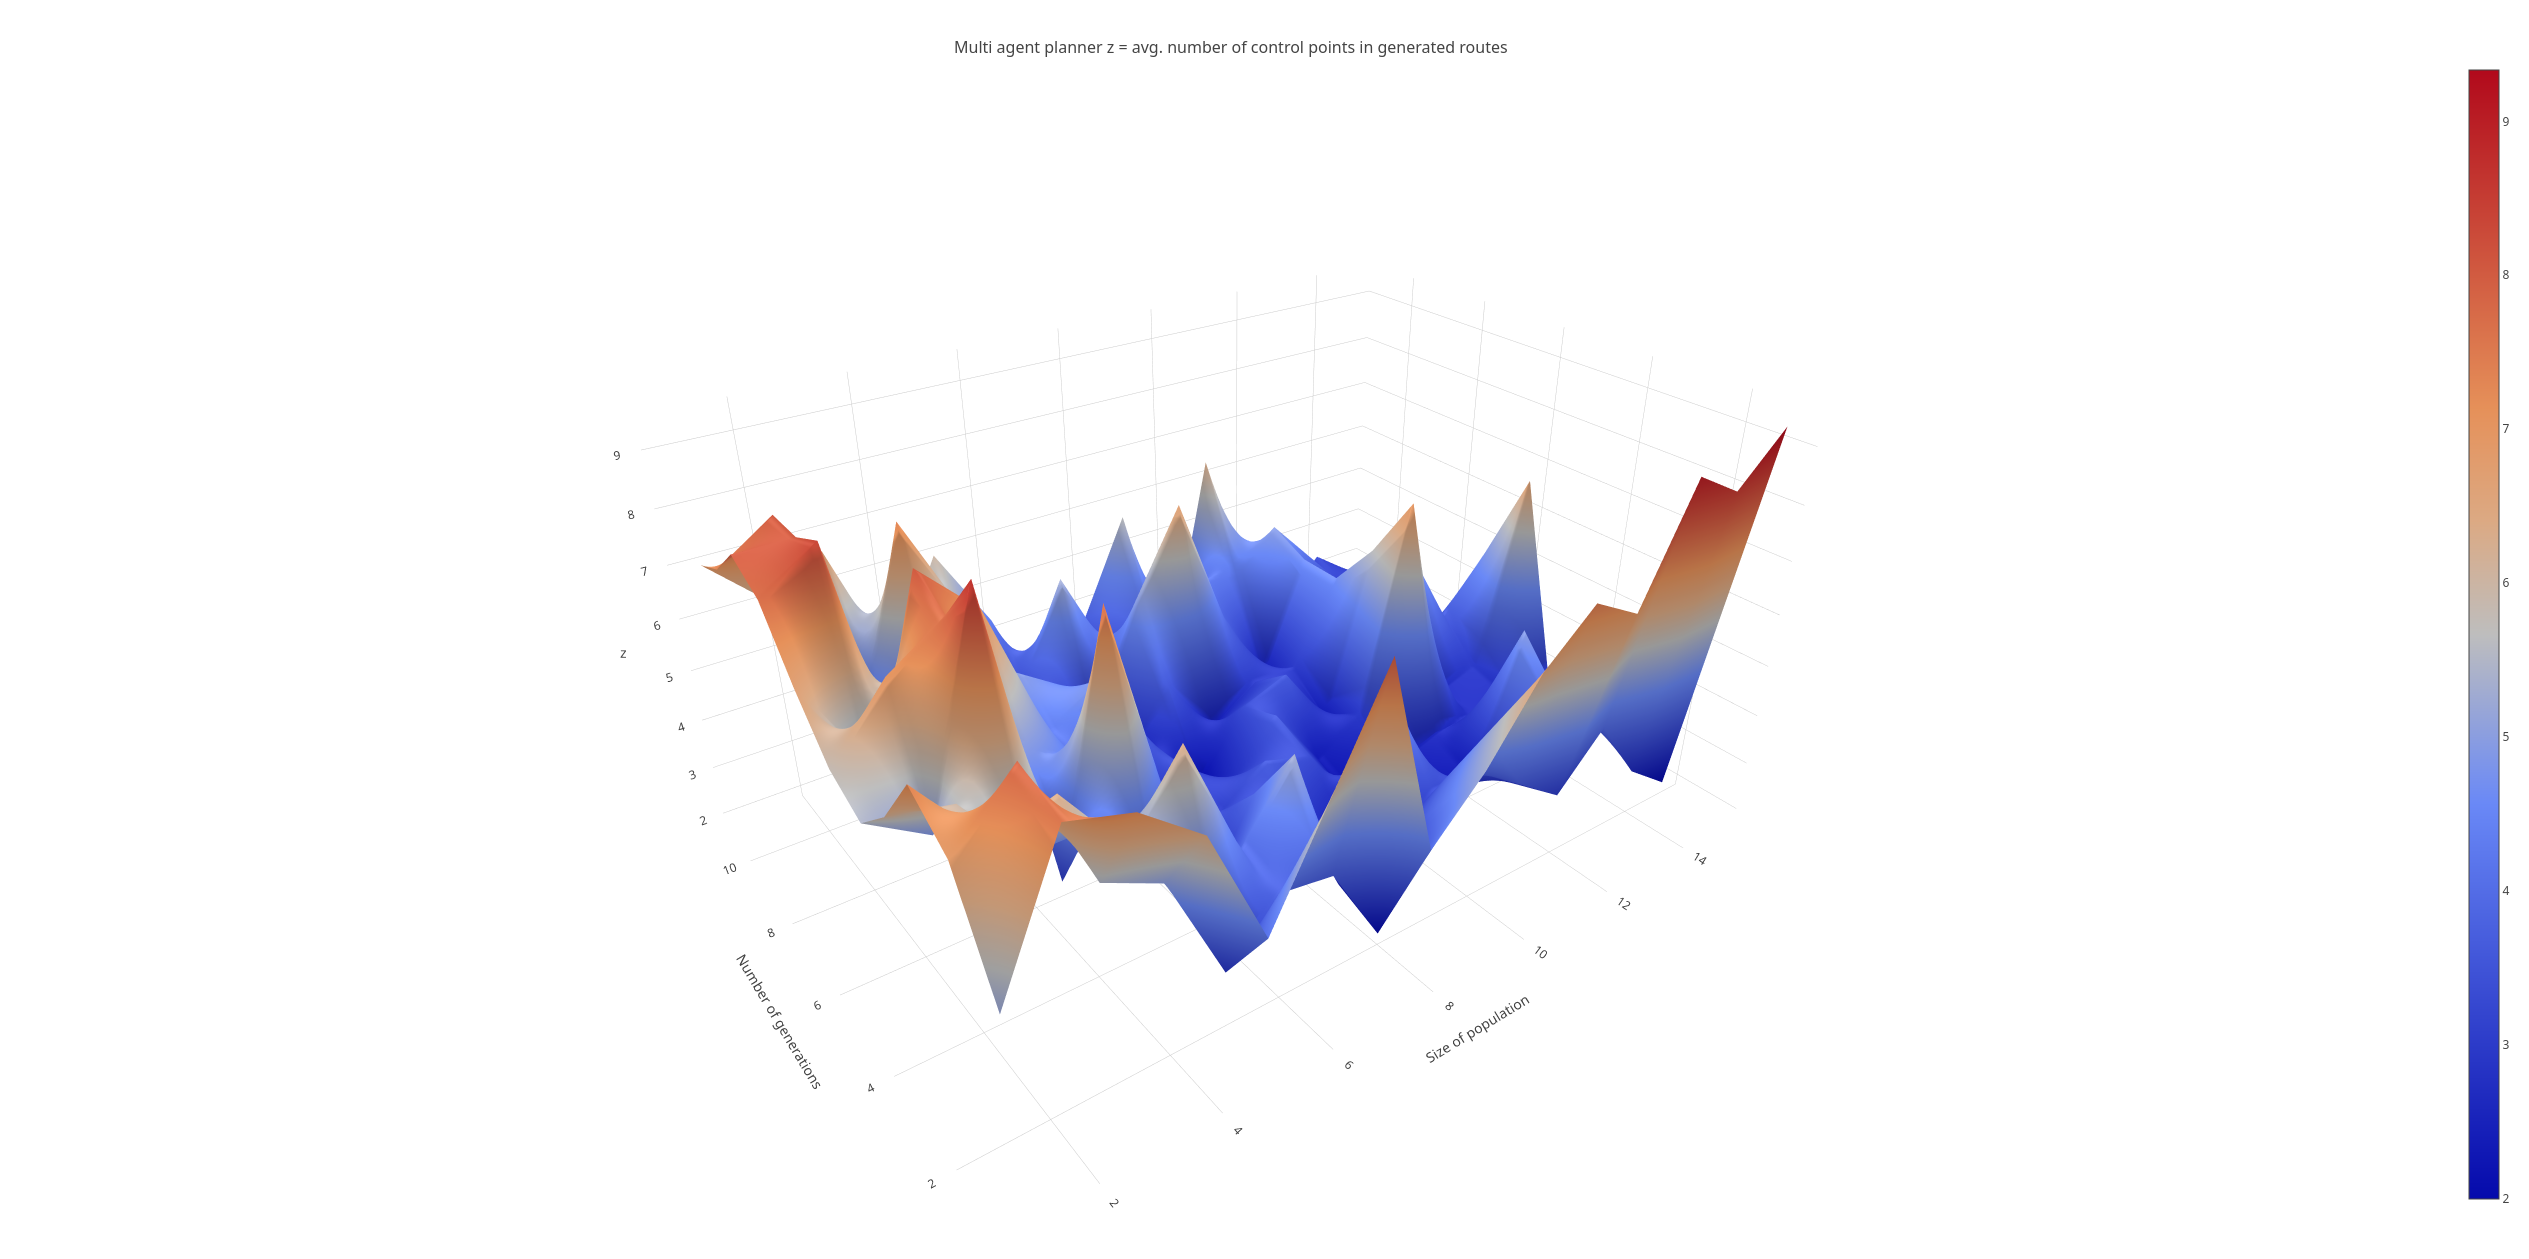
\includegraphics[width=\textwidth]{figures/ma-diff1-cps.png}
    \caption{\label{subfig:ma-diff1-cps}Average number of control points in routes for Road~\ref{subfig:ma-road1}}
  \end{subfigure}
  \begin{subfigure}[b]{0.44\textwidth}
    \centering
    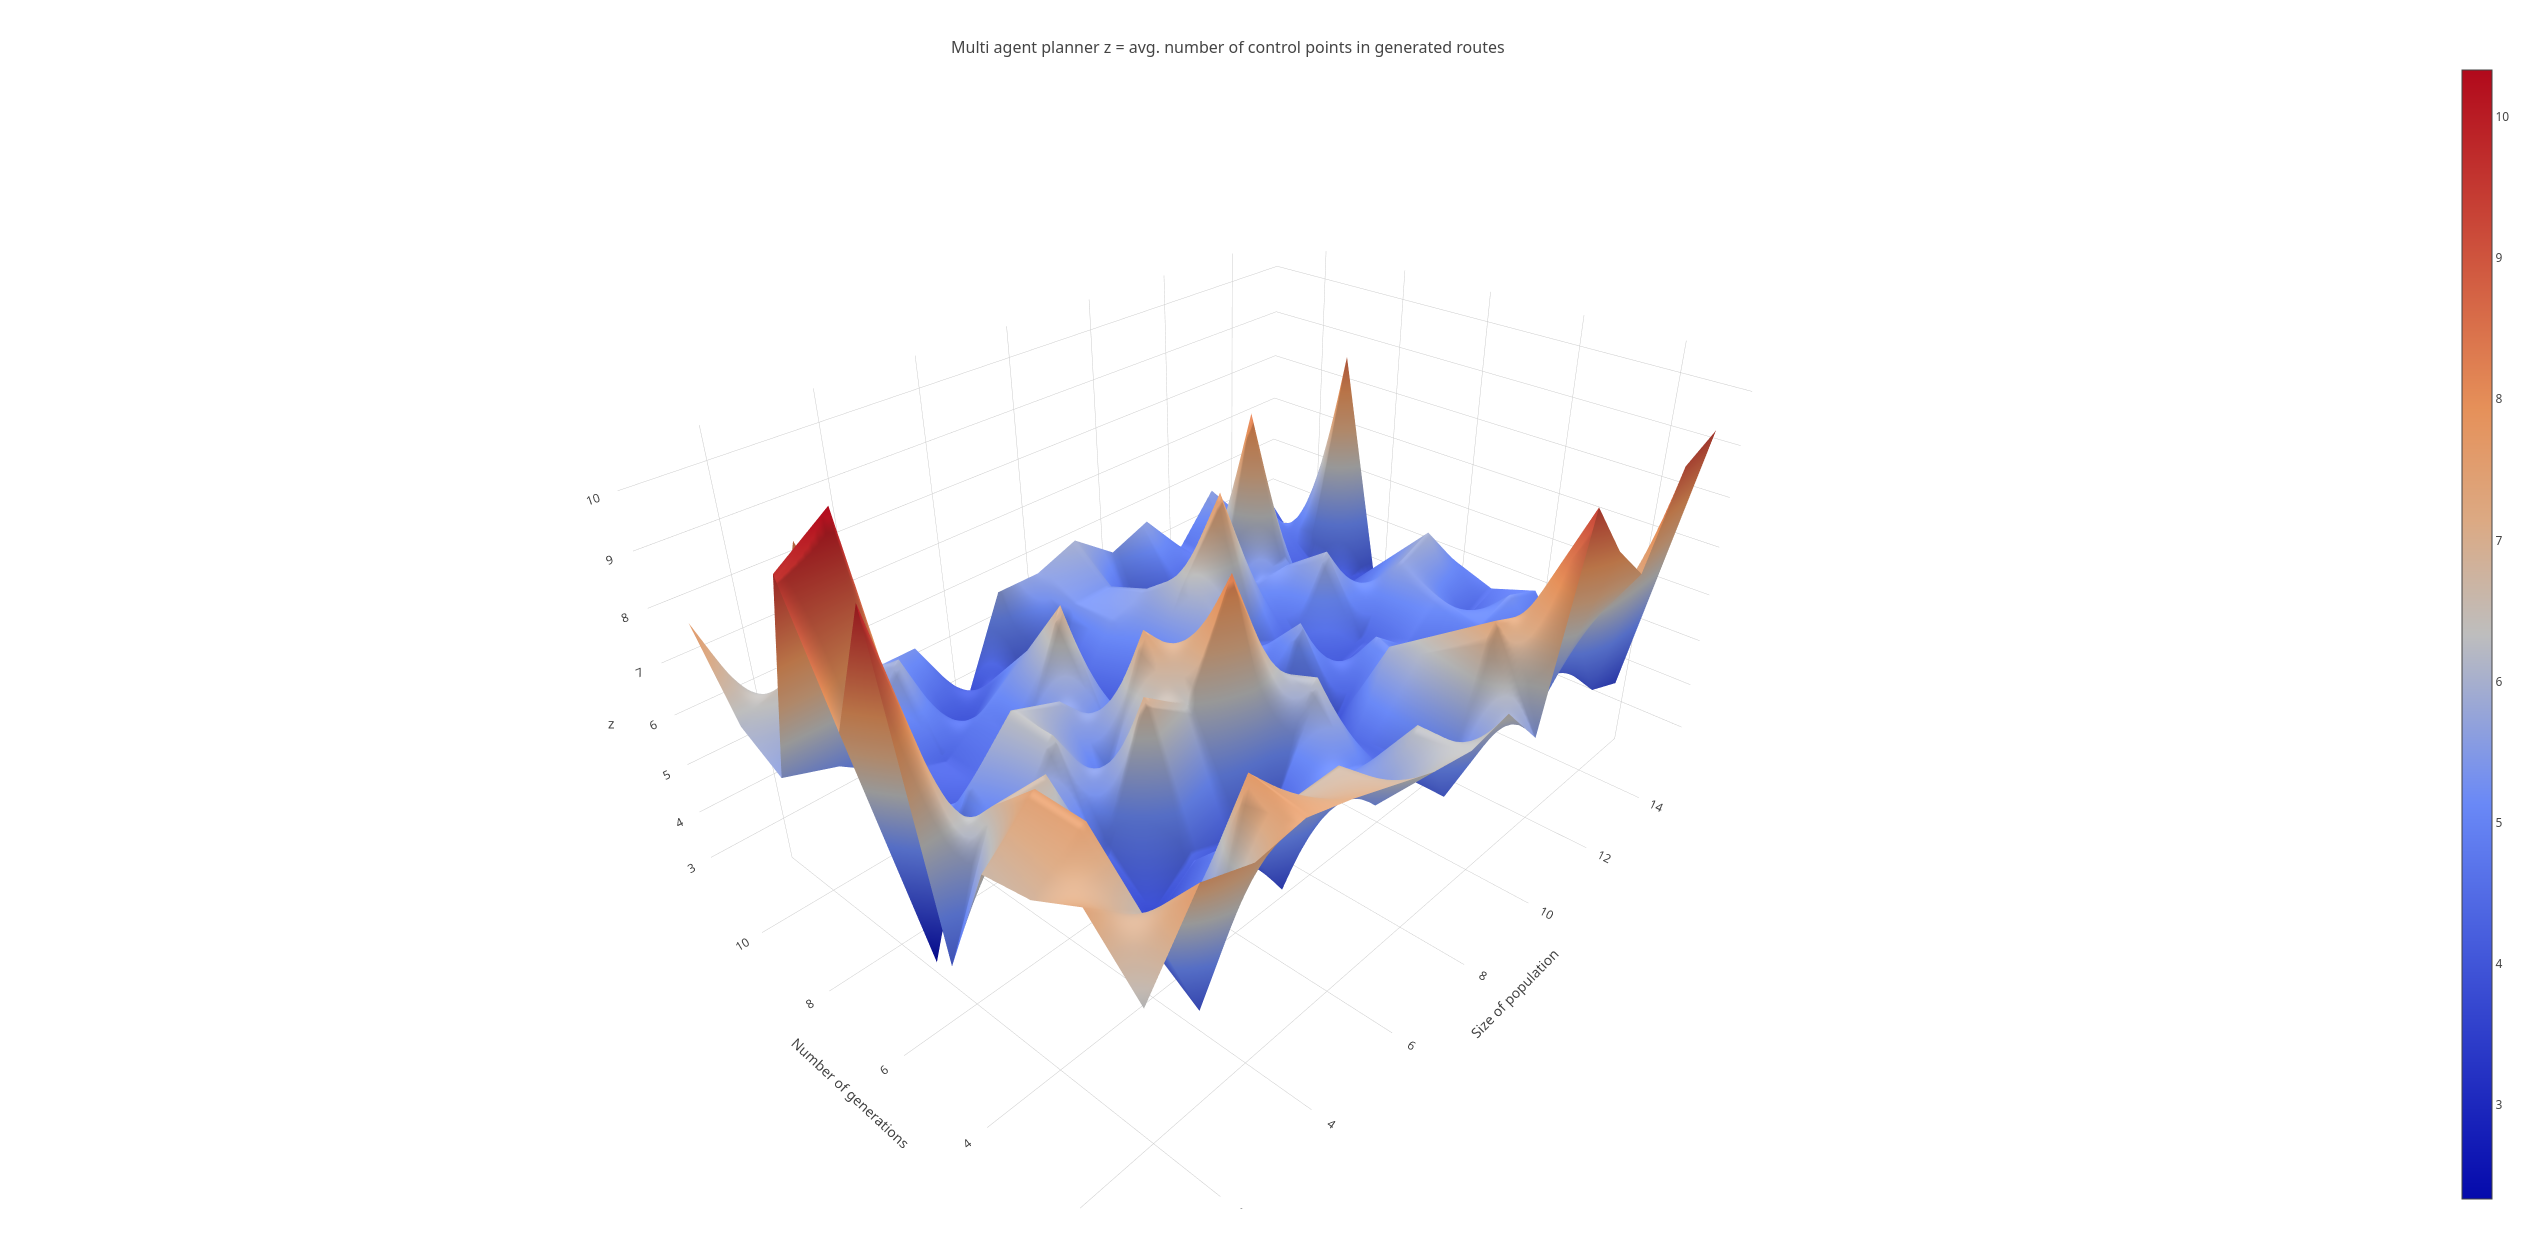
\includegraphics[width=\textwidth]{figures/ma-diff2-cps.png}
    \caption{\label{subfig:ma-diff2-cps}Average number of control points in routes for Road~\ref{subfig:ma-road2}}
  \end{subfigure}
  \begin{subfigure}[b]{0.44\textwidth}
    \centering
    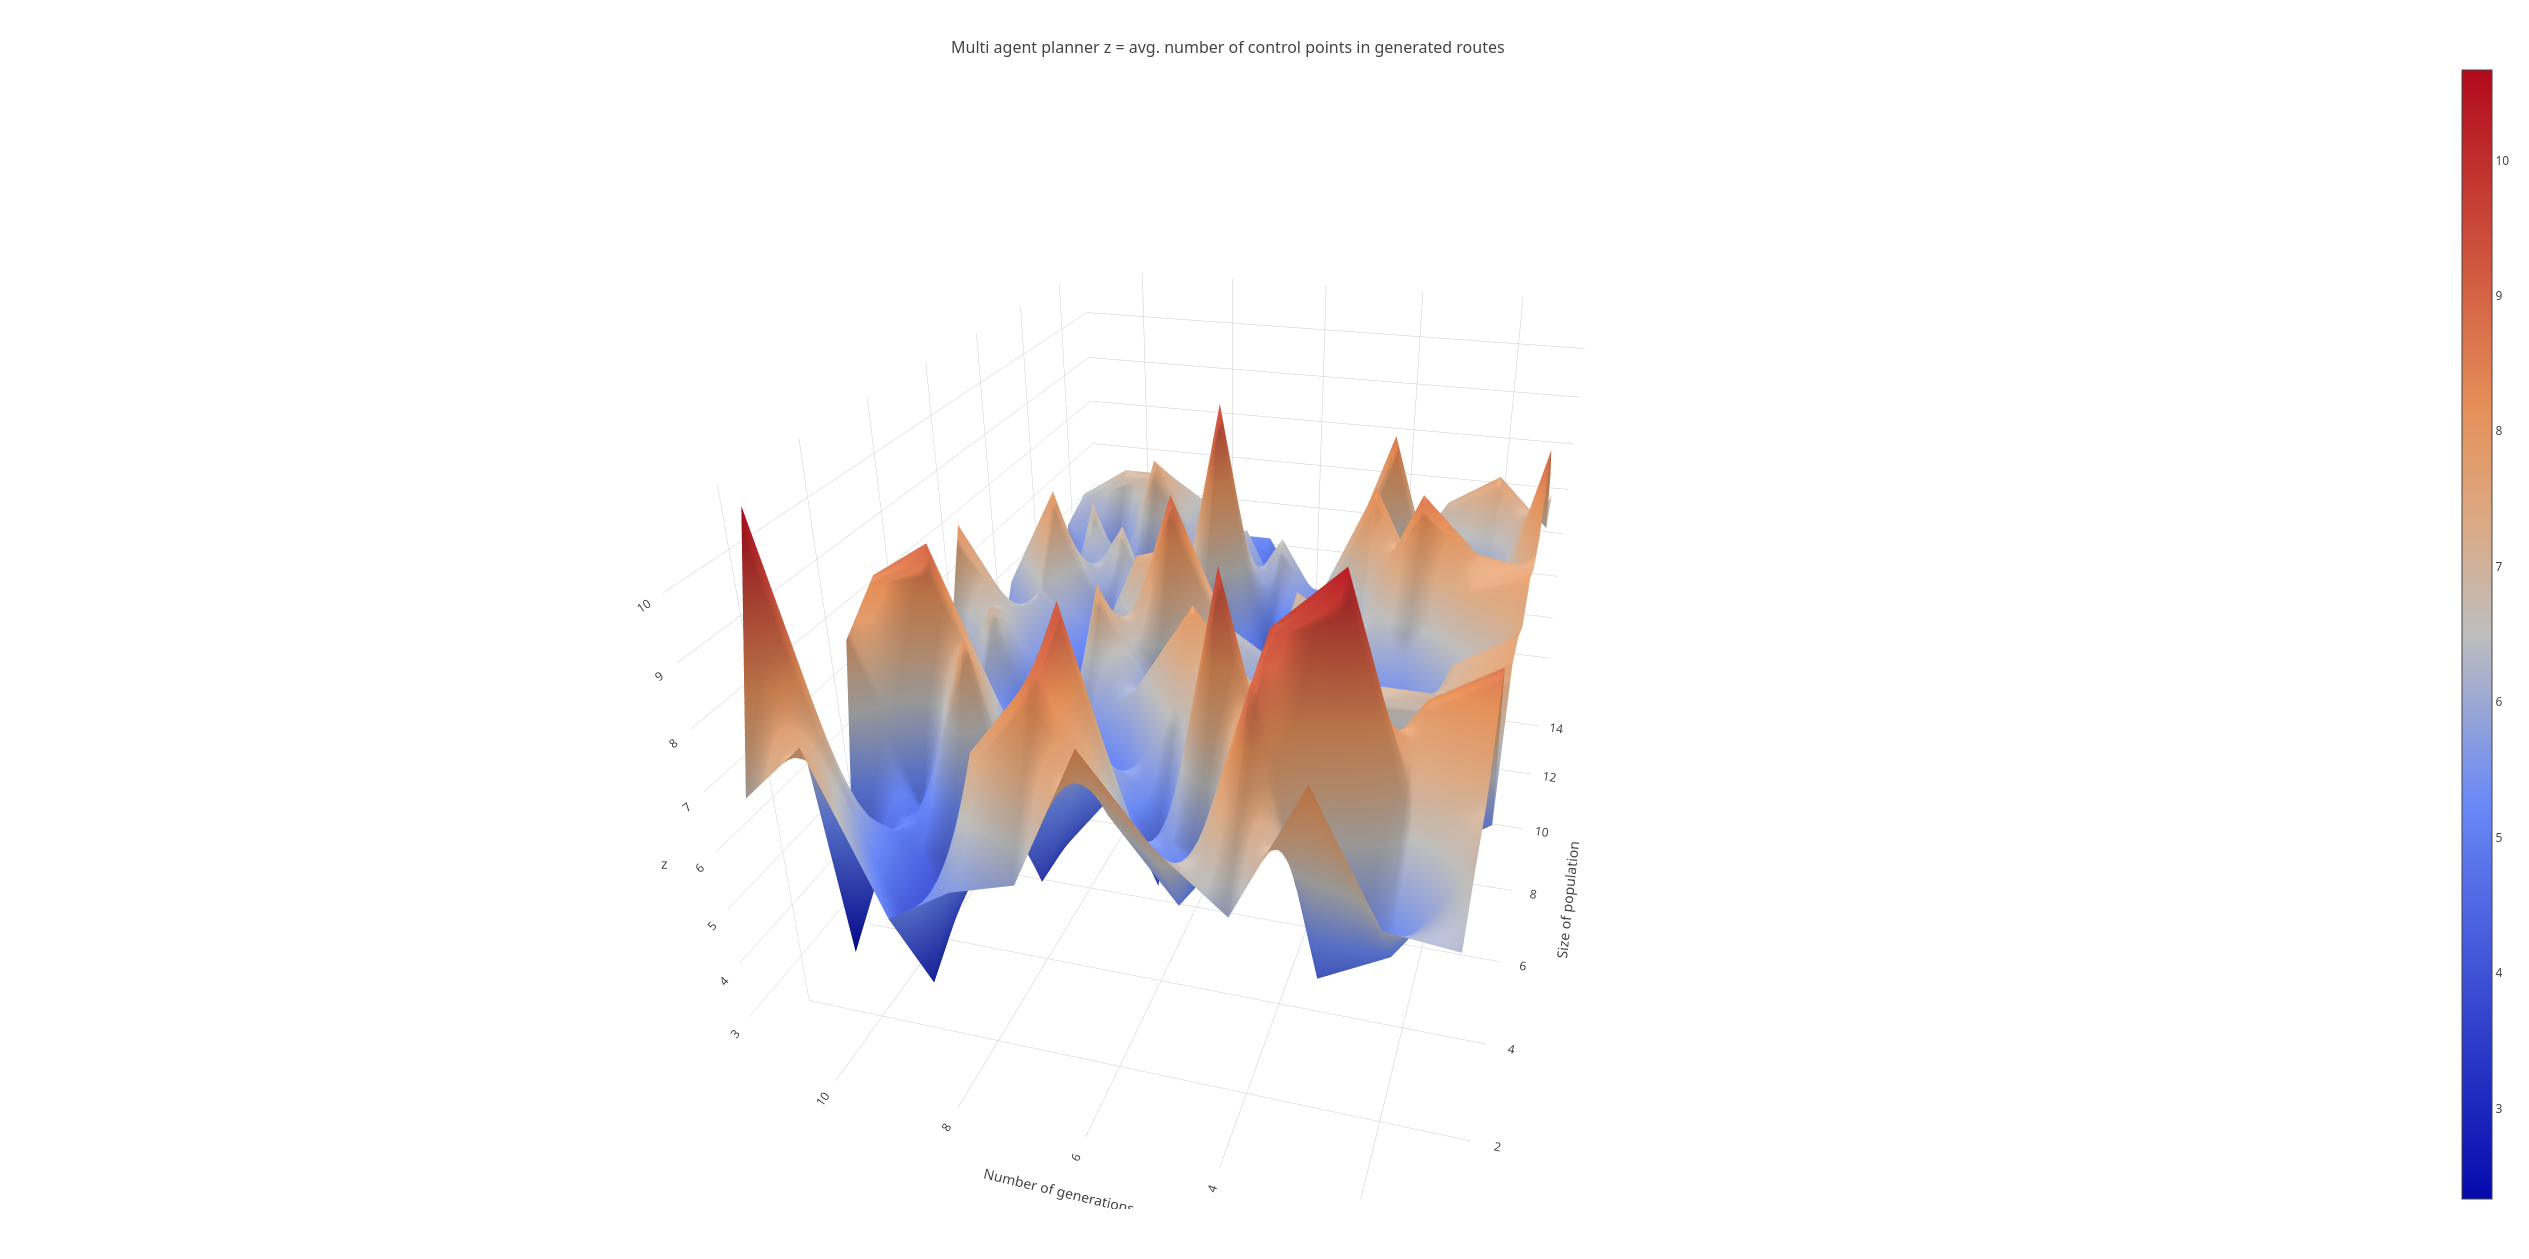
\includegraphics[width=\textwidth]{figures/ma-diff3-cps.png}
    \caption{\label{subfig:ma-diff3-cps}Average number of control points in routes for Road~\ref{subfig:ma-road3}}
  \end{subfigure}
  \begin{subfigure}[b]{0.44\textwidth}
    \centering
    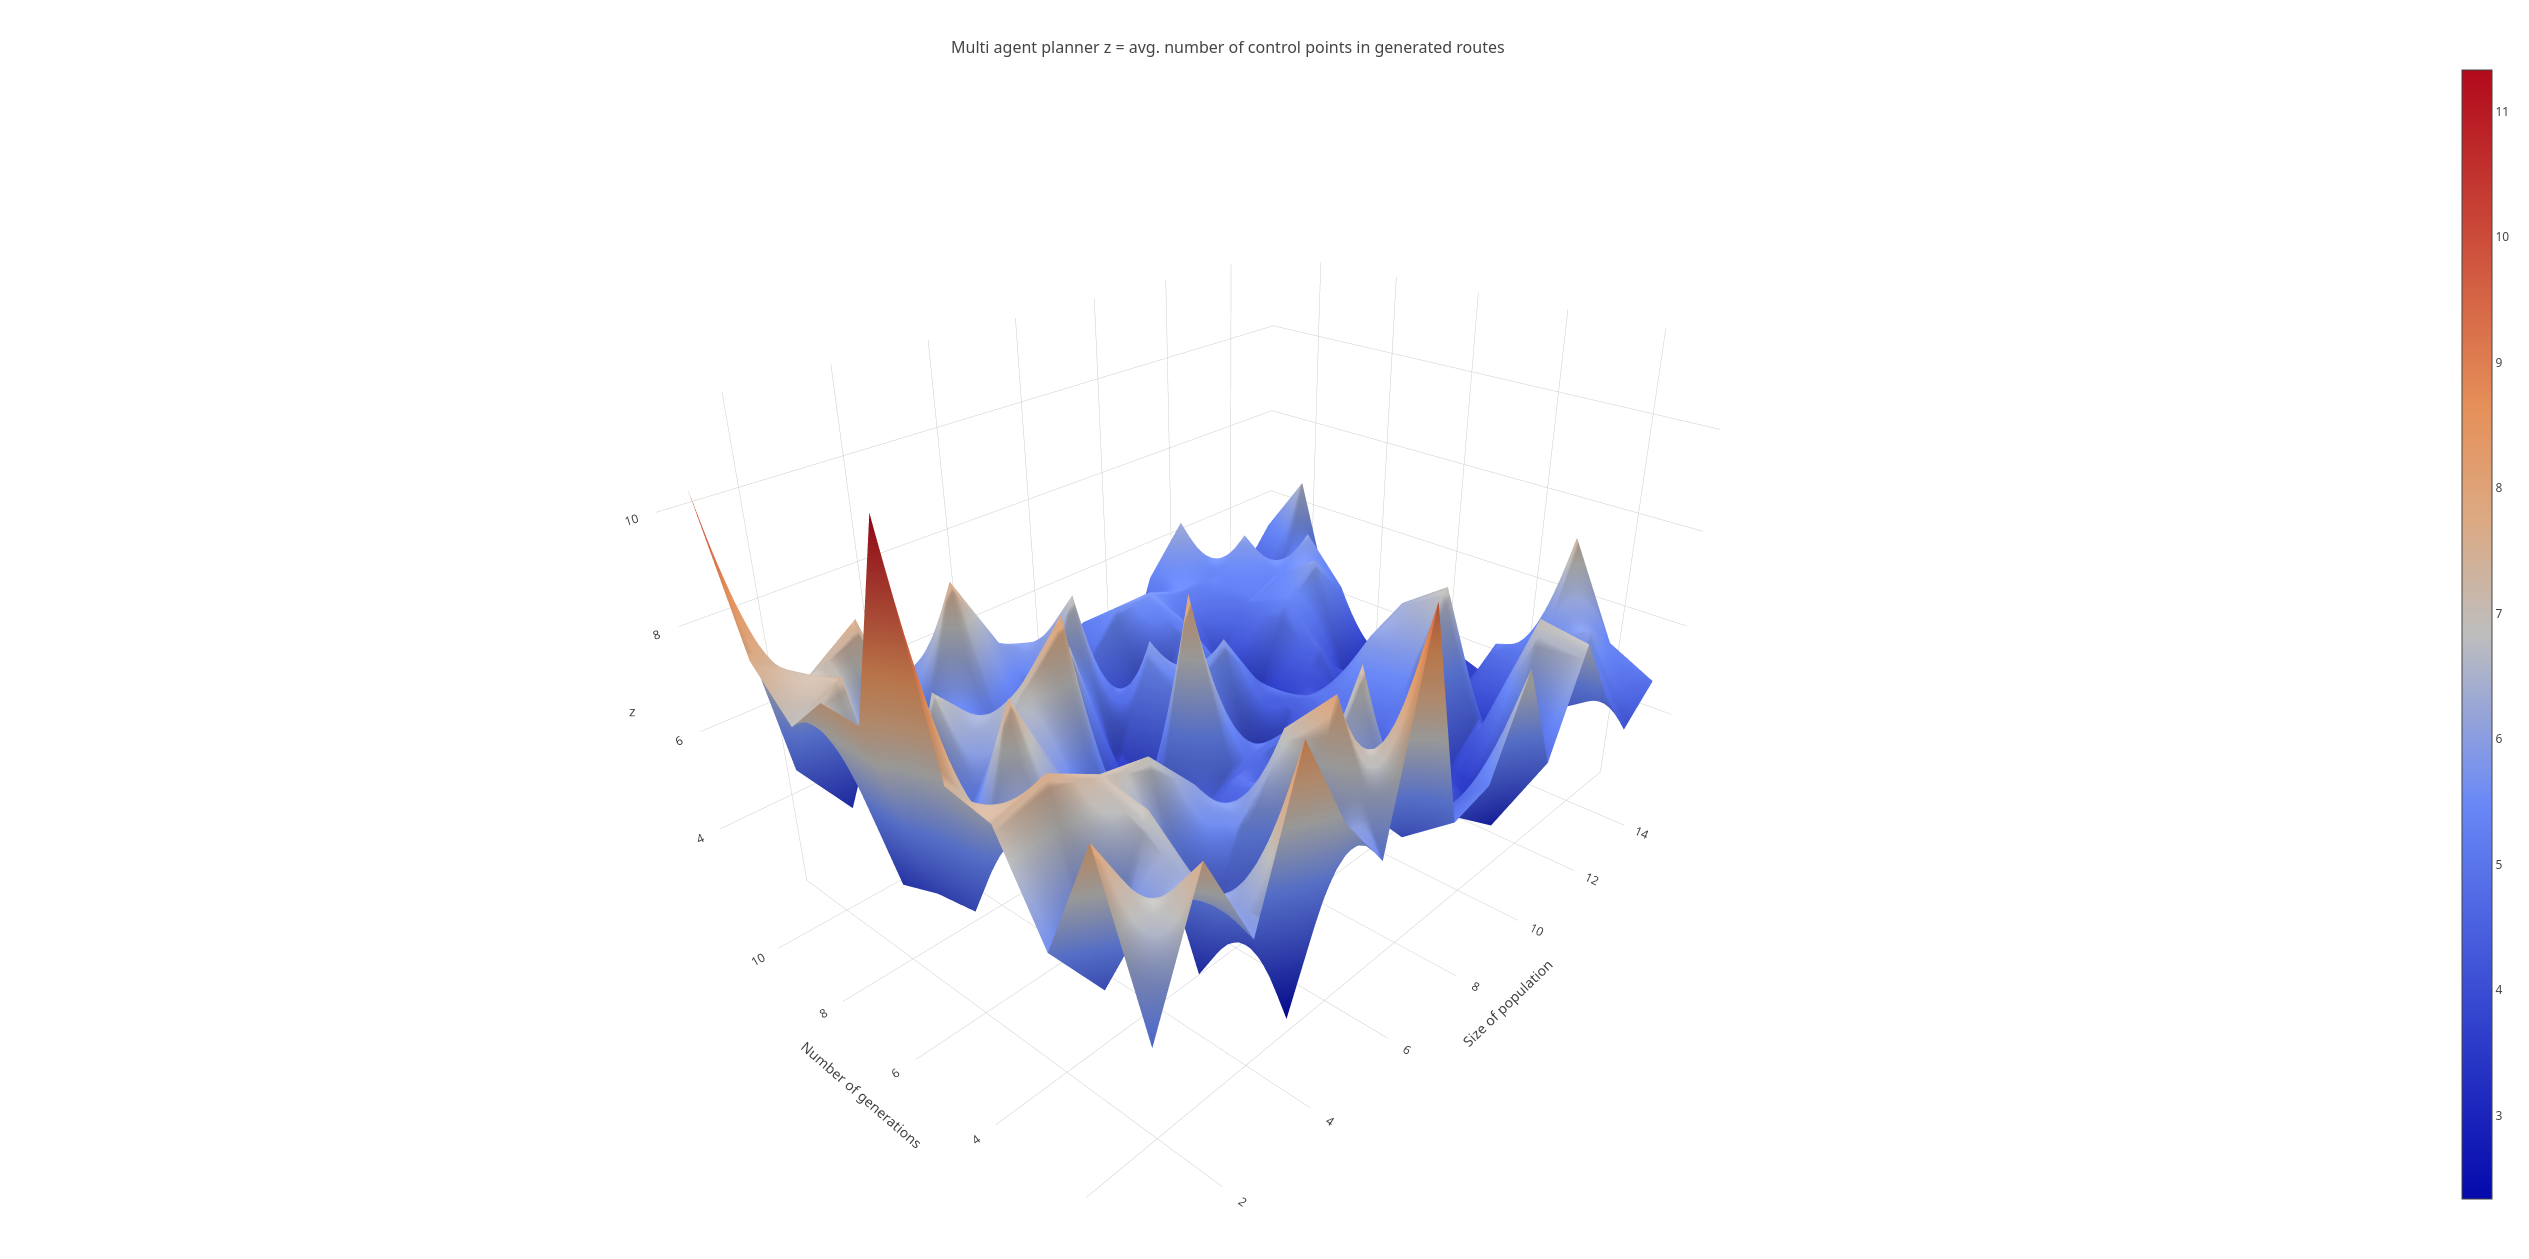
\includegraphics[width=\textwidth]{figures/ma-diff4-cps.png}
    \caption{\label{subfig:ma-diff4-cps}Average number of control points in routes for Road~\ref{subfig:ma-road4}}
  \end{subfigure}
  \caption{\label{fig:multi-agent-cps} Average solution complexity for a 3 agents over a varying number of generations and sizes of populations across various roads (See Figure~\ref{fig:multi-agent-roads}) }
\end{figure}

\todo{Check units for planning time + add link to hosted dynamic version}
\section{Macro-level Route planning}

The core of my macro-level planner was the previously evaluated multi-agent system, and as such I will not analyse its running time as the extra operations surrounding the invocations of the cooperative GA contribute relatively little time complexiy.

\section{Codebase Evaluation}

In total my codebase consists of around 2000 lines of Julia, a full breakdown can be seen in Figure~\ref{fig:codebase}\todo{is this figure required?}


\begin{figure}[ht]
  \centering
  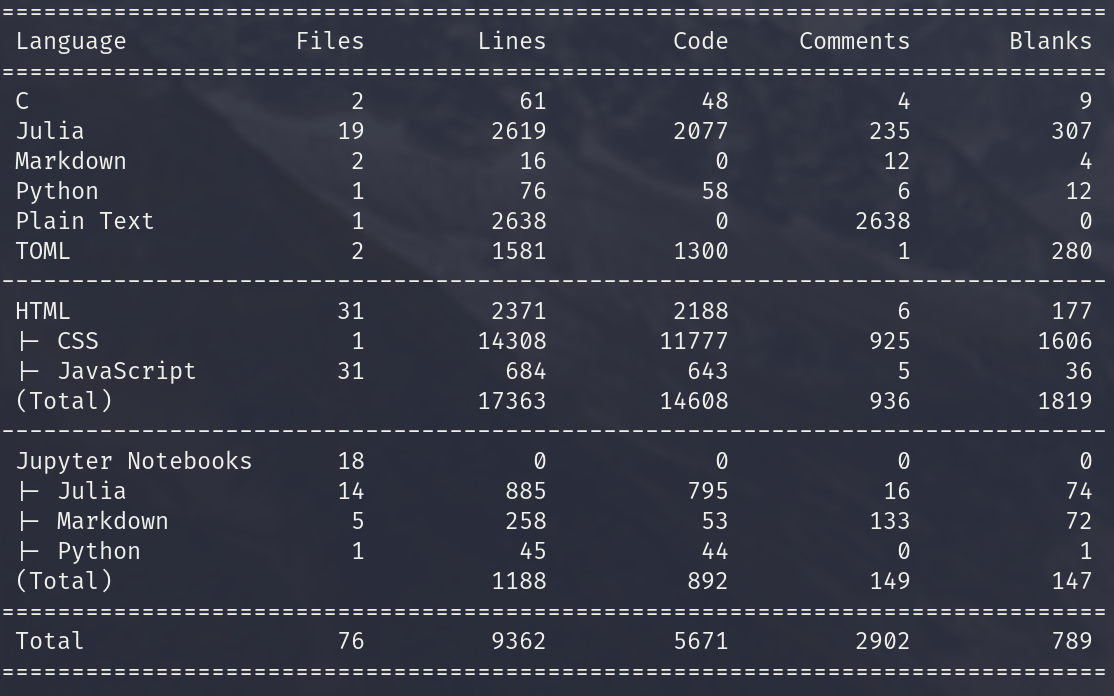
\includegraphics[scale=0.4]{figures/codebase.png}
  \caption{\label{fig:codebase} Codebase statistics, provided by tokei}
\end{figure}


%TC:macro \todo 1

%%% Local Variables:
%%% mode: latex
%%% TeX-master: "report"
%%% End:
